\documentclass[12pt,a4paper]{amsbook}
\usepackage{fullpage}
\usepackage{amssymb,amsfonts}
\usepackage{longtable}
\usepackage{graphicx}
\usepackage[export]{adjustbox}
\usepackage{cite}
\usepackage{subcaption}
\usepackage{amsmath}
\usepackage{placeins}
\renewcommand{\baselinestretch}{1.5}
\parskip10pt
\topmargin10mm
\oddsidemargin 0.07in
\textwidth 160 true mm
\textheight 225 true mm
\leftmargin=60mm
\usepackage{amsmath}

\newtheorem{theorem}{Theorem}%[chapter]
\newtheorem{lemma}[theorem]{Lemma}
\newtheorem{corollary}[theorem]{Corollary}
\newtheorem{proposition}[theorem]{Proposition}

\theoremstyle{definition}
\newtheorem{definition}[theorem]{Definition}
\newtheorem{remark}[theorem]{Remark}
\newtheorem{example}[theorem]{Example}
\newtheorem{problem}[theorem]{Problem}

\DeclareMathOperator{\arch}{arccosh}
\DeclareMathOperator{\arsh}{arcsinh}
\DeclareMathOperator{\diam}{diam}
\DeclareMathOperator{\card}{card}

\newcommand{\itemref}[1]{\ref{#1}}
\newcommand{\abs}[1]{\lvert #1\rvert}
\newcommand{\Rt}{{\mathbb R}^2}
\newcommand{\Rn}{{\mathbb R}^n}
\newcommand{\Rtbar}{\overline{{\mathbb R}^2}}
\newcommand{\Rnbar}{\overline{{\mathbb R}^n}}
\newcommand{\R}{{\mathbb R}}
\newcommand{\Rbar}{\overline{\mathbb R}}
\newcommand{\C}{{\mathbb C}}
\newcommand{\N}{{\mathbb N}}
\newcommand{\Q}{{\mathbb Q}}
\newcommand{\ch}{ \cosh }
\newcommand{\sh}{ \sinh }
\newcommand{\lqq}{\lq\lq}
\newcommand{\rqq}{\rq\rq\,}
\newcommand{\ident}{\equiv}
\newcommand{\abrv}{.\hskip 0.1truecm}
\renewcommand{\implies}{\Rightarrow}
\newcommand{\ineq}{\not =}
\newcommand{\superset}{\supset}
\newcommand{\ak}{\tilde{\alpha}}
\newcommand{\jk}{\tilde{j}}
\newcommand{\psubset}{\varsubsetneq}
\newcommand{\bibline}{\bysame}
\newcommand{\aeq}{\approx}
\newcommand{\ale}{\lesssim}
\newcommand{\age}{\gtrsim}
\newcommand{\mle}{\ll}
\newcommand{\mge}{\gg}
\newcommand{\notcomp}{\lessgtr}
\newcommand{\ip}[2]{<\!\!#1, #2\!\!>}
\newcommand{\MA}{\operatorname{MA}}
\newcommand{\HMA}{\operatorname{HMA}}
\newcommand{\HC}{\operatorname{HC}}
\newcommand{\Cc}{\overline{\mathbb{C}}} %Riemann sphere
%-------------------------------------------------------
%------------------------------------------------------



\begin{document}
\thispagestyle{empty}
% \begin{figure}
% %\vspace{-10cm}
% \begin{center}
% %\vspace*{-9.5cm}
% \includegraphics{emblem1.ps}
% \end{center}
% \caption{Hi}
% \end{figure}
% \begin{center}
% {\epsfig{file=emblem1.ps, scale=1.0}}
% \end{center}
\begin{center}
{\large\bf  CLAS-ANALYSIS NOTE}
\end{center}
\vspace*{.8cm}
\begin{center}
{ Dalitz Plot Analysis of $\eta^{\prime}$ $\rightarrow$ $\eta$ $\pi^{+}$ $\pi^{-}$ from CLAS G12 Data Set}
\end{center}
%\vspace*{.4cm}

%\begin{center}
%{\it to be submitted in partial fulfillment of the\\
%requirements for the award of the degree}
%\end{center}
\vspace*{.6cm}
%\centerline{ \bf {\em of}}
%\centerline{\large\bf DOCTOR OF PHILOSOPHY}
\vspace*{.8cm}
%\centerline{\it by}
%\centerline{\large\bf NAME OF THE STUDENT}
%\vspace*{1.3cm}
%\centerline{\it for the award of the degree}
%\vspace*{.4cm}
%\centerline{\it of}
%\vspace*{.4cm}
%\centerline{\large\bf DOCTOR OF PHILOSOPHY}
\vspace{3cm}
%\centerline{\includegraphics[width=3.8cm]{logo-iiti-1.eps}}
%\medskip
\vspace{.8cm}
\begin{center}\large\bfseries

%M.P.-- 452 020
\end{center}
\vspace*{.5cm}
%\centerline{\bf MONTH AND YEAR OF SUBMISSION}



\bibliographystyle{plain}
\pagestyle{plain}
%\pagenumbering{roman}
% \newpage
 \thispagestyle{empty}

\newpage
\setcounter{page}{1}


%%%%%%%%%%%%%%%%%%%%%%%%%%%%%%%%
%%%%%%%%%%% section 1 %%%%%%%%%%
%%%%%%%%%%%%%%%%%%%%%%%%%%%%%%%%
\section{Introduction}

The present work aims to report the Dalitz plot parameters for $\eta^{\prime}$ $\rightarrow$ $\eta$ $\pi^{+}$ $\pi^{-}$ decay. The three body decay of a meson has two degrees of freedom, so one can define a Dalitz plot with two variables X and Y for $\eta^{\prime}$ $\rightarrow$ $\eta$ $\pi^{+}$ $\pi^{-}$ decay, which is defined as follows:

\begin{eqnarray}
X&=&\frac{\sqrt{3}(T_{\pi^{+}} -T_{\pi^{-}})}{Q} \\ 
Y&=&\frac{(m_{\eta}+2m_{\pi})}{m_{\pi} }\cdot \frac{T_{\eta}}{Q} - 1.
\end{eqnarray}

Where $T_{\eta}$, $T_{\pi^{+}}$ and $T_{\pi^{-}}$ are the kinetic energy of a given particles $\eta$, $\pi^{+}$ and $\pi^{-}$ respectively in the rest frame of $\eta^{\prime}$ and Q = $T_{\pi^{+}}$+$T_{\pi^{-}}$+$T_{\eta}$. The $m_{\eta}$ and $m_{\pi}$ are the mass of  $\eta$ and $\pi$ mesons respectively. 

\begin{figure}[ht!]
\centerline{
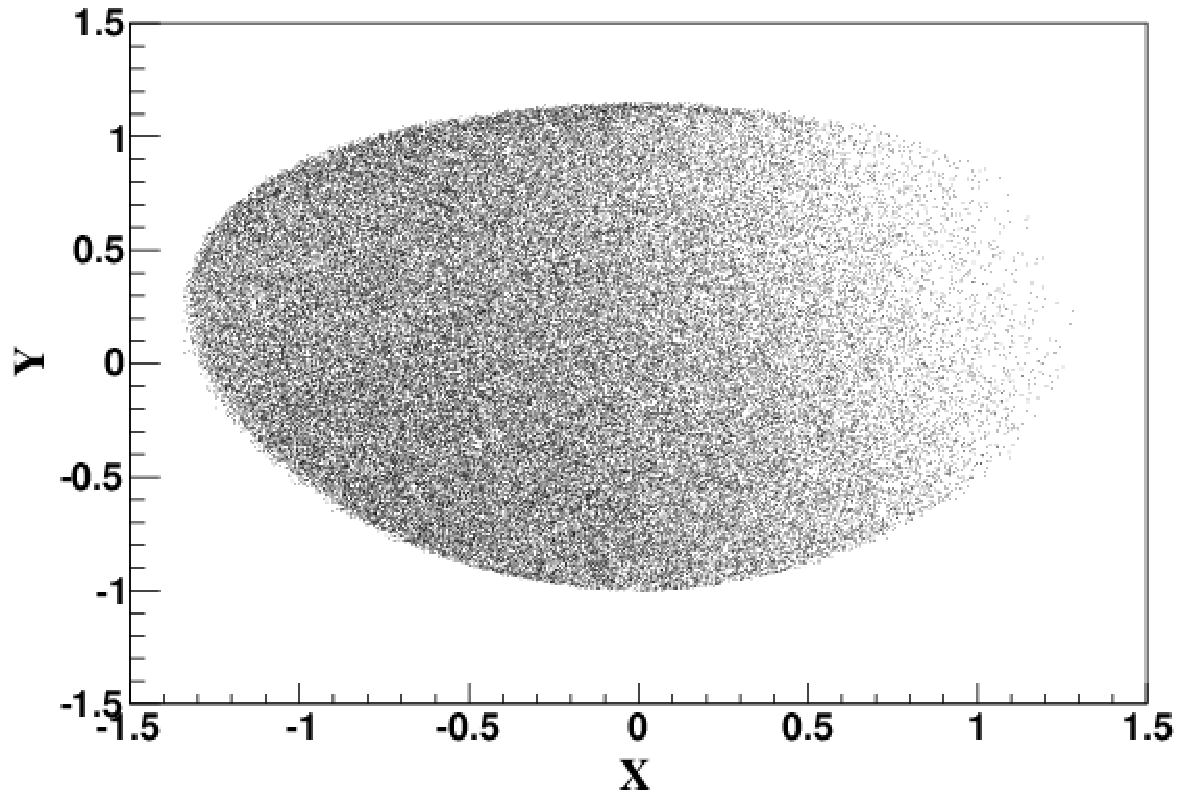
\includegraphics[width=12cm,height=8cm]{dalitzEtaPrime.pdf}}
\caption{Dalitz variable X vs Y for $\eta^{\prime}$ $\rightarrow$ $\eta$ $\pi^{+}$ $\pi^{-}$.}
\label{DP}
\end{figure}

The general parametization function in Equation.~\ref{par} is used to fit a Dalitz plot. The square of the decay amplitude,
 \begin{equation}
M^{2}=A(1+aY+bY^{2}+cX+dX^{2}).
\label{par}
\end{equation}
Where a, b, c, and d are the Dalitz plot parameters of the decay and A is the normalization constant.

The Dalitz plot(DP) provides pure kinematic information of a three body decay and also helps to understand the correct input to theoretical distribution of the effective chiral Lagrangian. A Dalitz plot study for the $\eta^{\prime}$ meson for the $\eta$ $\pi^{+}$ $\pi^{-}$  decay channel will help to study effective chiral perturbation theory at a low Q limit.

The VES Collaboration has reported the Dalitz plot parameters of $\eta^{\prime}$ $\rightarrow$ $\eta$ $\pi^{+}$ $\pi^{-}$ with 14.6 x $10^{3}$ events in charge exchange and 7 x $10^{3}$ events in diffraction like production ~\cite{Dorofeev:2006fb}. The BESIII Collaboration has also reported $\eta^{\prime}$ $\rightarrow$ $\eta$ $\pi^{+}$ $\pi^{-}$ decay parameters with 43826 ± 211 events with better precision~\cite{Ablikim:2010kp}. The two measurements has disagreement among them and also to the theoretical calculation of the parameters ~\cite{Borasoy:2005du}. 

In this note the Dalitz plot parameters of $\eta^{\prime}$ $\rightarrow$ $\eta$ $\pi^{+}$ $\pi^{-}$ is studied with CLAS g12 data set, which has the competitive statistics to study the parameters with low statistical errors. It is yet another independent measurement with different systematic errors to cross-check the parameters.

\section {G12 Data Set}

The g12 experiment ran during March - June 2008 with 26 x $10^{9}$ recorded production triggers ~\cite{G12_AN}.  The fixed target g12 experiment, has an energy of the photon beam ranging from 1.142 GeV to  5.425 GeV. However the threshold production of $\eta^{\prime}$ meson is 1.455 GeV and hence the analysis will report the parameters from the threshold to the maximum available energy. The analysis starts with well calibrated data in ".root" format with all events arranged as per the Run number, Event number and PID along with all other informations recorded by the experiment. The final state particles proton, $\pi^{+}$ and $\pi^{-}$ information were extracted from the PART BOS bank and identified using particle identification codes compiled in the ``clas6-trunk" under the package CLASEVENT . The skim were so selected that all events has only one proton, $\pi^{+}$ and $\pi^{-}$ and any number of neutral particles. 
The complete reaction under study is `` $\gamma$ p $\rightarrow$ $\eta^{\prime}$($\rightarrow$ $\eta$ $\pi^{+}$ $\pi^{-}$) p " and the $\eta$ meson is detected via the missing mass technique. 

\subsection{Run List}
The g12 experiment recorded 626 production runs, 37 single-prong runs and 3 special calibration runs. The Table.~\ref{RunList} shows the list of runs used in the analysis.

\begin{longtable}{|c|c|c|c|c|}
\caption{List of runs included in the analysis}\\
\hline
G12 Run List &G12 Run List & G12 Run List & G12 Run List & G12 Run List \\
\hline
56605&56653&56654&56655&56656\\ 
56660&56661&56665&56666&56667\\ 
56668&56669&56670&56673&56674\\ 
56688&56689&56690&56691&56692\\ 
56693&56694&56695&56696&56700\\ 
56701&56702&56703&56704&56705\\ 
56706&56707&56708&56710&56711\\ 
56712&56713&56714&56715&56716\\ 
56717&56718&56719&56720&56721\\ 
56722&56723&56724&56726&56727\\ 
56728&56729&56730&56731&56732\\ 
56733&56734&56735&56736&56737\\ 
56738&56739&56740&56741&56742\\ 
56743&56744&56748&56749&56750\\ 
56751&56752&56753&56754&56755\\ 
56756&56757&56758&56759&56760\\ 
56761&56762&56763&56764&56765\\ 
56766&56767&56768&56770&56771\\ 
56772&56774&56775&56776&56777\\ 
56778&56780&56781&56782&56783\\ 
56784&56787&56788&56791&56792\\ 
56793&56794&56798&56799&56800\\ 
56801&56802&56805&56806&56807\\ 
56808&56809&56810&56811&56812\\ 
56813&56814&56815&56821&56822\\ 
56823&56824&56825&56826&56827\\ 
56831&56832&56833&56834&56838\\ 
56839&56841&56842&56843&56844\\ 
56845&56849&56853&56854&56855\\ 
56856&56857&56858&56859&56860\\ 
56861&56862&56864&56865&56866\\ 
56870&56874&56875&56877&56879\\ 
56897&56898&56899&56900&56901\\ 
56902&56903&56904&56905&56907\\ 
56908&56914&56915&56916&56917\\ 
56918&56919&56921&56922&56923\\ 
56924&56925&56926&56927&56928\\ 
56929&56930&56932&56935&56936\\ 
56937&56938&56939&56940&56948\\ 
56949&56950&56951&56952&56953\\ 
56954&56955&56956&56958&56960\\ 
56961&56962&56963&56964&56965\\ 
56966&56967&56968&56969&56970\\ 
56971&56972&56973&56974&56975\\ 
56977&56978&56979&56980&56992\\ 
56993&56994&56996&56997&56998\\ 
56999&57000&57001&57002&57003\\ 
57004&57005&57006&57008&57009\\ 
57010&57011&57012&57013&57014\\ 
57015&57016&57017&57021&57022\\ 
57023&57025&57026&57027&57030\\ 
57031&57032&57062&57063&57064\\ 
57065&57066&57067&57068&57069\\ 
57071&57072&57073&57075&57076\\ 
57077&57078&57079&57080&57095\\ 
57096&57097&57100&57101&57102\\ 
57103&57106&57107&57108&57114\\ 
57115&57116&57117&57118&57119\\ 
57120&57121&57122&57123&57124\\ 
57125&57126&57127&57128&57130\\ 
57131&57132&57133&57134&57135\\ 
57136&57137&57138&57139&57140\\ 
57141&57142&57143&57144&57145\\ 
57146&57147&57148&57149&57150\\ 
57151&57152&57159&57160&57161\\ 
57162&57163&57164&57165&57166\\ 
57167&57168&57170&57171&57172\\ 
57173&57174&57175&57176&57177\\ 
57178&57179&57180&57181&57182\\ 
57183&57184&57185&57189&57190\\ 
57191&57192&57193&57194&57195\\ 
57196&57197&57198&57199&57200\\ 
57201&57202&57203&57204&57205\\ 
57206&57207&57208&57209&57210\\ 
57211&57212&57213&57214&57215\\ 
57216&57217&57218&57219&57220\\ 
57221&57222&57223&57224&57225\\ 
57226&57227&57228&57229&57233\\ 
57234&57235&57236&57249&57250\\ 
57251&57252&57253&57255&57256\\ 
57257&57258&57260&57261&57262\\ 
57263&57264&57265&57266&57267\\ 
57268&57270&57271&57272&57274\\ 
57275&57276&57277&57278&57279\\ 
57280&57281&57282&57283&57284\\ 
57285&57286&57287&57288&57290\\ 
57291&57293&57294&57295&57296\\ 
57297&57298&57299&57300&57301\\ 
57302&57303&57304&57305&57306\\ 
57307&57308&57309&57310&57311\\ 
57317&57308&57309&57310&57311\\ 
\hline
\label{RunList}
\end{longtable}


The whole analysis is divided into following sections.
\begin {itemize}
\item Simulation 
\item Event Selection 
\item Result 
\item Systematics Study
\end {itemize}



%%%%%%%%%%%%%%%%%%%%%%%%%%%%%%%%
%%%%%%%%%%% section 3 %%%%%%%%%%
%%%%%%%%%%%%%%%%%%%%%%%%%%%%%%%%
\subsection{Simulation}
\label{Sim}
PLUTO++, an event generator is used for this analysis. It uses ROOT based programmes and it is very commonly used in Hadron Physics experiments to generate hadronic production and decay of mesons. It gives user the freedom to include physics models with simple C++ based codes and to obtain outputs in any desired format. The simulated events in the analysis are modelled with bremsstrahlung photon, differential cross-section of $\eta^{\prime}$ ~\cite{Williams:2009yj} and Dalitz plot parameters of $\eta^{\prime}$ $\rightarrow$ $\eta$ $\pi^{+}$ $\pi^{-}$ decay. The output of the PLUTO++ program are extracted in standard CLAS ``gamp" file and then processed with CLAS simulation suit in the following way :

\begin {itemize}
\item The gamp files are first converted into the format of PART bank containing the event.
\item GSIM:  Geant3-based simulation in CLAS simulates the decay tracks of particles through the simulation and finally the digitized informations is sorted in the simulated ``raw" banks.
\item GPP: GSIM post-processor smears detector signal more accurately to reflect the actual resolution and to simulate the experimental conditions.  
\item a1c : It is used for reconstruction of simulated data and is the same program used during data reconstruction.
\end {itemize}

\section{Event Selection}

This section explains the procedure to improve the identification of the particles, corrections to the event and cuts to the analysis. 

\subsection{Selection of the Beam Photon}

A typical g12 data event has multiple bremsstrahlung photons recorded as the incident beam. The multiple beam photon arises from 2.004 beam bunching spacing of the electrons in the storage ring. These electrons gives the bremsstrahlung photons in the radiator and creates multiple hits in the trigger and thereby satisfying trigger logic to record them. All the  photons which falls within the timing window of $\mid$Tagger Time - StartTime$\mid$ $\leq$ 1.002 ns are considered as an individual event.

\subsection{G12 Corrections}
\label{Cor}
The G12 Corrections were derived from the exclusive $\pi^{+}$, $\pi^{-}$ and proton reaction. We used the following corrections in the analysis ~\cite{G12_AN}:
    
\begin {itemize}
\item Beam Energy Correction : Is a correction to the incident beam photon energy and dependent on the Run number of the event. This correction is only applicable data and not to the simulated events.
\item Removal of bad TOF paddle : This correction takes the Sector number and Paddle number as input. We used the correction to remove only those paddles that shows a significant drift on the resolutions of particle.   
\item  Geometric Fiducial Cut : This cut removes the dead part of the detector from the $\theta-\phi$ map of the particle. We used it with the "nominal" option. 
\end {itemize}

\subsection{Kinematic Fitting}
\label{KF}
Kinematic fitter is a useful tool often used to get rid of unwanted background from signal channels and helps to improve the signal to background ratio.  Any measurement with a tool comes with an error, and it can be represented as a vector  $\vec{\eta}$. We can also define the measurement as 
\\ $\vec{\eta}$ =  $\vec{y}$. +  $\vec{\epsilon}$.\\
Where the $\vec{y}$ and $\vec{\epsilon}$ denotes the actual value of the measurement without error and $\vec{\epsilon}$ is the error associated with the measurement. The kinematic information of a physics channel along with the constrains imposed allows the fitter to calculate the probability and $\chi^{2}$ of each event using Lagrange multipliers to perform a least-squares fit. The CLAS g12 Kinematic fitter takes the ``TBER (Track Based Error)" matrix, vertex of information and four-momentum of all particles as input, and returns Pull probabilities and $\chi^{2}$ for each events. The Pull probabilities when fitted with Guassian, its mean and $\sigma$ decides the quality of the covariance matrix and kinematic fit. In the ideal case of gaussian fitted to the Pulls of the particles should have  zero mean and $\sigma$ of one, which ensures that the fitter correctly calculates covariance matrix error. 
  
\begin{figure}[ht!]
\centerline{
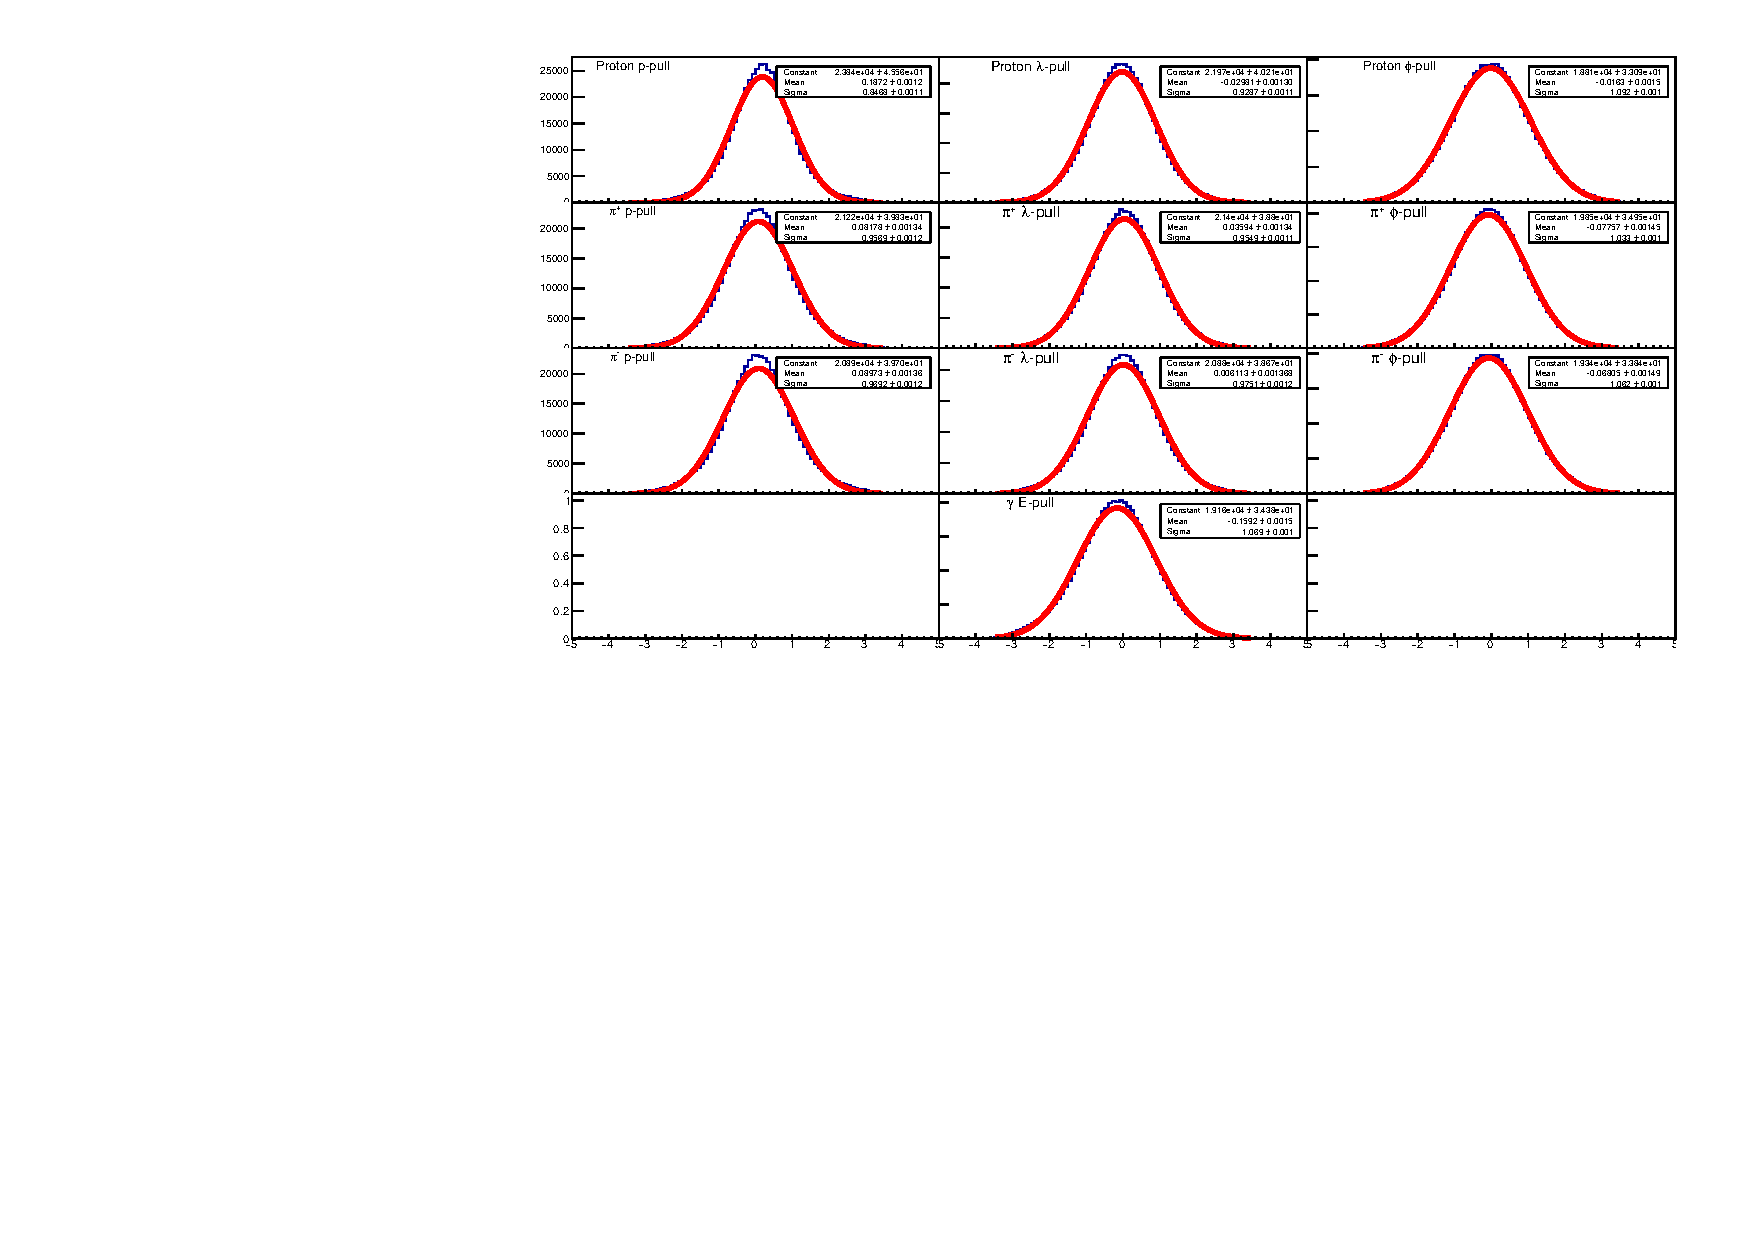
\includegraphics[width=12cm,height=10cm]{Pulls_nothing.pdf}}
\caption{The Pull distributions for a (4-C) kinematic fit to $\gamma$ p $\rightarrow$ $\pi^{+}$ $\pi^{-}$ p from g12 data with run 56655 after a 1$\%$ Pull probability cut.}
\label{Fig3}
\end{figure}

\begin{figure}[ht!]
\centerline{
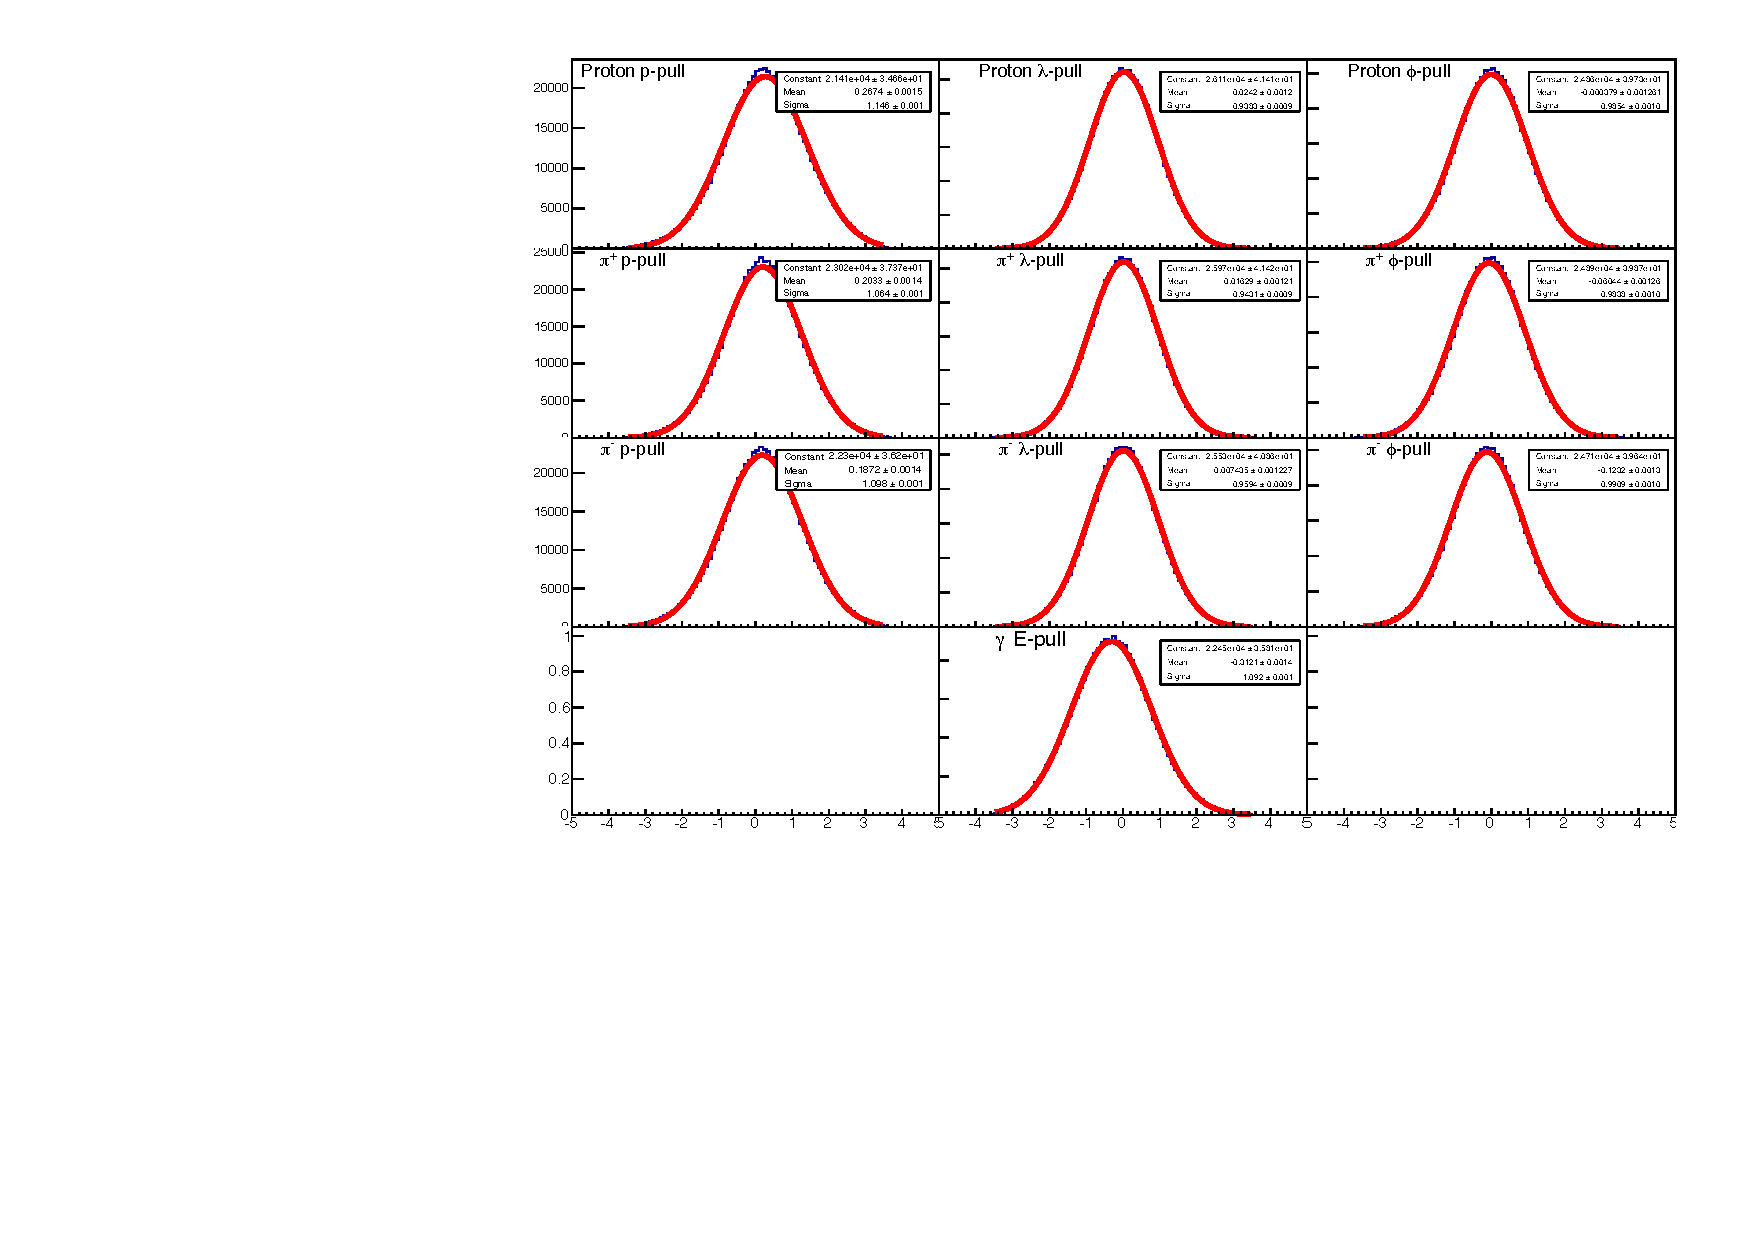
\includegraphics[width=12cm,height=10cm]{SIM_Pulls_nothing.pdf}}
\caption{The Pull distributions for a (4-C) kinematic fit to $\gamma$ p $\rightarrow$ $\pi^{+}$ $\pi^{-}$ p from g12 simulation after a 1$\%$ Pull probability cut.}
\label{Fig4}
\end{figure}
  
The CLAS g12 Kinematic fitter is tuned for 4C constrained reaction,

\begin{eqnarray*}
\gamma p \rightarrow \pi^{+} \pi^{-} p.
\end{eqnarray*}\\
\noindent
The tuning were done for $\pi^{+}$ $\pi^{-}$ and p individually. To check the quality of covariance matrix the mean and sigma of the tuned pulls of the particles $\pi^{+}$, $\pi^{-}$ and p from the reaction hypothesis for the data with run 56655 and simulation after a 1$\%$ pull probability cut is listed in the Table.~\ref{tab2}.

\begin{table}
\centering
\begin{subtable}{.5\textwidth}
\centering
\caption{ }
\begin{tabular}{ |c|c|c| }
\hline
                                                &$\mu$   &$\sigma$ \\
                               \hline
Proton p-pull                            & 0.187  & 0.846  \\
\hline
Proton $\lambda$-pull                      & -0.029 & 0.928  \\
\hline
Proton $\phi$-pull                         & -0.016 & 1.092  \\
\hline
$\pi^{+}$ p-pull        & 0.081  & 0.957  \\
\hline
$\pi^{+}$ $\lambda$-pull & 0.035  & 0.954  \\
\hline
$\pi^{-}$ $\phi$-pull    & -0.077 & 1.033  \\
\hline
$\pi^{-}$ p-pull        & 0.089  & 0.969  \\
\hline
$\pi^{-}$ $\lambda$-pull & 0.006  & 0.975  \\
\hline
$\pi^{-}$ $\phi$-pull    & -0.068 & 1.062  \\
\hline
$\gamma$ E-pull   & -0.159 & 1.069 \\
\hline
\end{tabular}
\end{subtable}%
\begin{subtable}{.5\textwidth}
\centering
\caption{ }
\begin{tabular}{ |c|c|c| }
\hline
                                         &$\mu$   &$\sigma$ \\ \hline
Proton p-pull                             & 0.267  & 1.146  \\
\hline
Proton $\lambda$-pull                  & 0.024  & 0.938  \\
\hline
Proton $\phi$-pull                         & -0.000 & 0.985  \\
\hline
$\pi^{+}$ p-pull        & 0.203  & 1.064  \\
\hline
$\pi^{+}$ $\lambda$-pull & 0.016  & 0.943  \\
\hline
$\pi^{+}$ $\phi$-pull    & -0.060 & 0.983  \\
\hline
$\pi^{-}$ p-pull        & 0.187  & 1.098  \\
\hline
$\pi^{-}$ $\lambda$-pull & 0.007  & 0.959  \\
\hline
$\pi^{-}$ $\phi$-pull    & -0.123 & 0.990  \\
\hline
$\gamma$ E-pull                           & -0.312 & 1.092  \\ 
\hline
\end{tabular}
\end{subtable}%
\caption{The table shows the Gaussian mean ($\mu$) and width ($\sigma$) for the pull distributions from a 4C kinematic fit of  $\gamma$ p $\rightarrow$ $\pi^{+}$ $\pi^{-}$ to events from (A) data run 56655 and (B) from simulation after a 1$\%$ Pull probability cut.} 
\label{tab2}
\end{table}

\subsubsection{Kinematic Fit to the Analysis}
	
\begin{figure}[ht!]
\centerline{
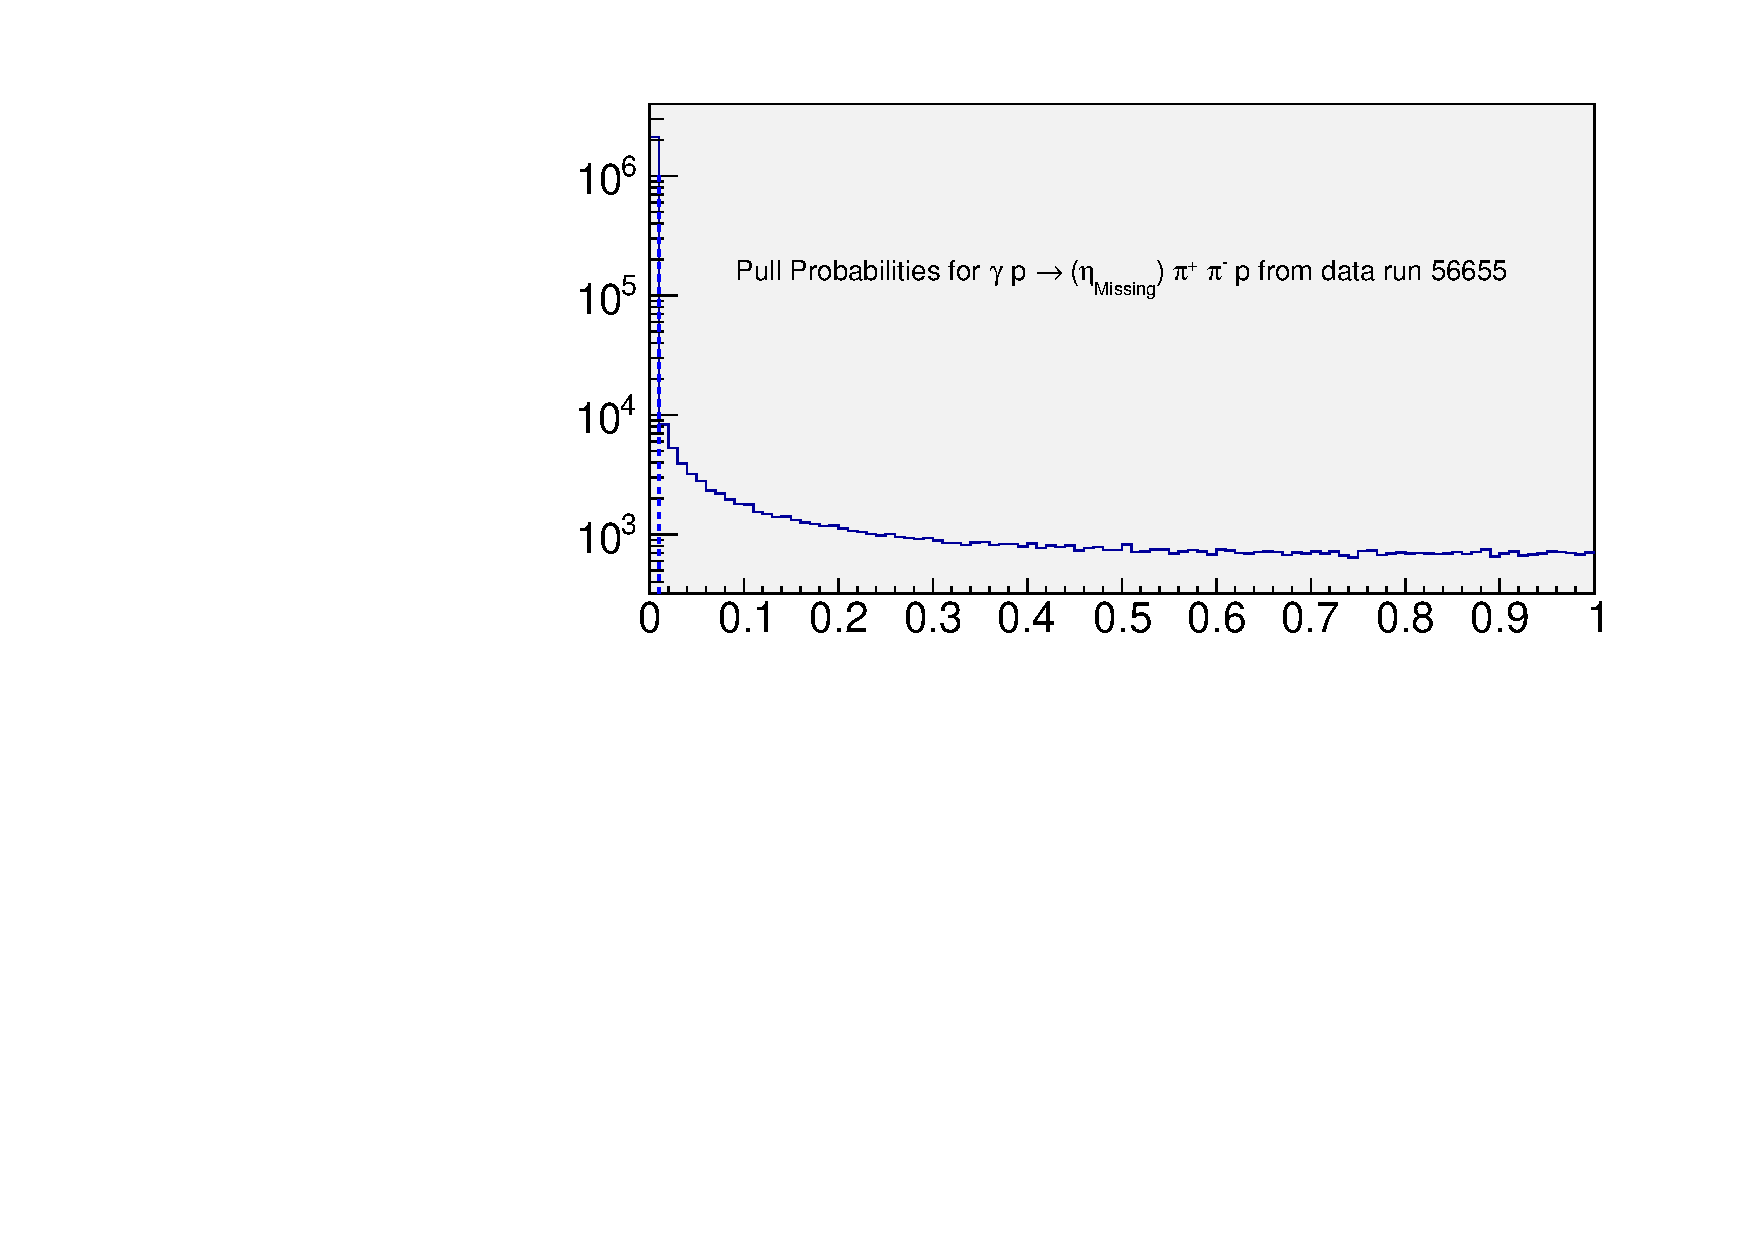
\includegraphics[width=12cm,height=8cm]{Prob_etafit.pdf}}
\caption{The Pull probability for a (1C) kinematic fit to $\gamma$ p $\rightarrow$ ($\eta_{Missing})$ $\pi^{+}$ $\pi^{-}$ p from data run 56655.}
\label{Fig5}
\end{figure} 

The tuned Kinematic fitter for the 4C constrained fit is again used for the channel below
\begin{eqnarray*}
\gamma p \rightarrow (\eta)_{Missing} \pi^{+} \pi^{-} p. (1C)
\end{eqnarray*}\\	
 The 1-C constrained fit requires the four-momentum [beam] + [target] - ( [$\pi^{+}$] [$\pi^{-}$] [p]) to be an [$\eta$] meson. The reaction hypothesis has the same set of final state particles as for the tuned channel, hence one can comfortably use it without tuning it for our reaction hypothesis again. The Pull probability for the channel is shown in Fig.~\ref{Fig5} and the dotted line at 0.01 shows the 1$\%$ Pull probability cut to reject events. 

\subsection{$\mid$ $\cos\theta_{center-of-mass}$ of $\eta^{\prime}$ $\mid$ $\leq$ 0.85 Cut}
\label{Cos}


The events are generated with the differential cross sections of $\eta^{\prime}$ from the g11 measurement ~\cite{Williams:2009yj} within a $\mid$ $\cos\theta_{center-of-mass}$ of $\eta^{\prime}$ $\mid$ $\leq$ 0.85. The earlier measurement of CLAS g11 has reported the differential cross sections in $\mid$ $\cos\theta_{center-of-mass}$ of $\eta^{\prime}$ $\mid$ $\leq$ 0.85 window as the yield drops near to the beam pipe and hence this region is removed from the analysis.  

\subsection{$\mid$ $\cos\theta_{center-of-mass}$ of $\eta$ $\mid$ $\leq$ 0.85 Cut}
\label{CosEta}

  The $\eta$ mesons along the beam pipe in the forward and backward region is removed with a condition requiring $\mid$ $\cos$ $\theta_{center-of-mass}$ of $\eta$ $\mid$ $\leq$ 0.85.  The Figure.~\ref{Fig_CsE_1} shows the $\cos$($\theta$) distribution of $\eta$ meson in the rest frame of $\eta^{\prime}$ meson for both data and simulation. The Figure.~\ref{Fig_CsE_2} clearly shows the steep drop of acceptance for the $\eta$ meson with high kinetic energy decaying along the beam pipe region. Hence the a geometrical cut at $\mid$ $\cos$ $\theta_{center-of-mass}$ of $\eta$ $\mid$ $\leq$ 0.85 is placed in order to calculate integrated acceptance for Dalitz plot parameters. 
  
 \begin{figure}[ht!]
\centerline{
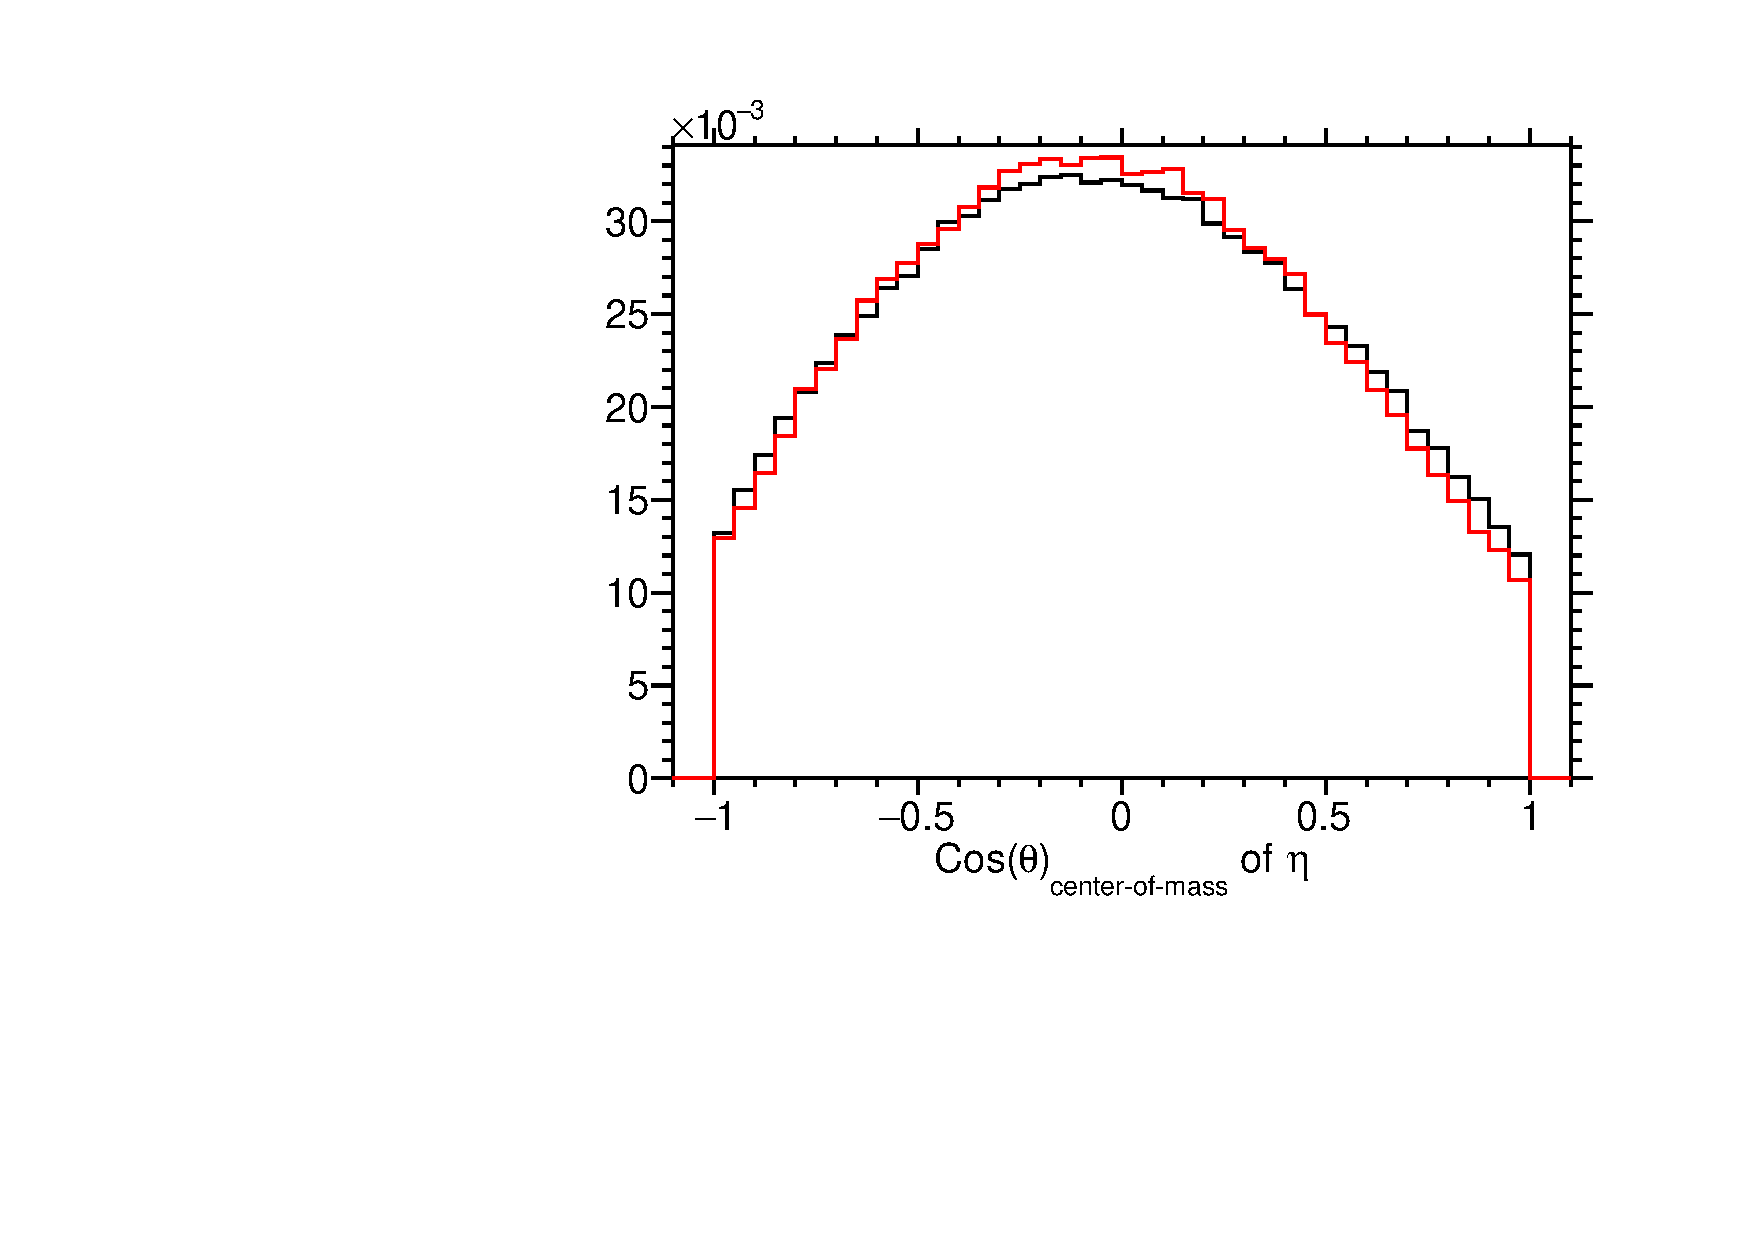
\includegraphics[width=12cm,height=8cm]{cs.pdf}}
\caption{$\cos\theta_{center-of-mass}$ of $\eta$ distribution from g12 data and simulation. }
\label{Fig_CsE_1}
\end{figure}


\begin{figure}[ht!]
\centerline{
%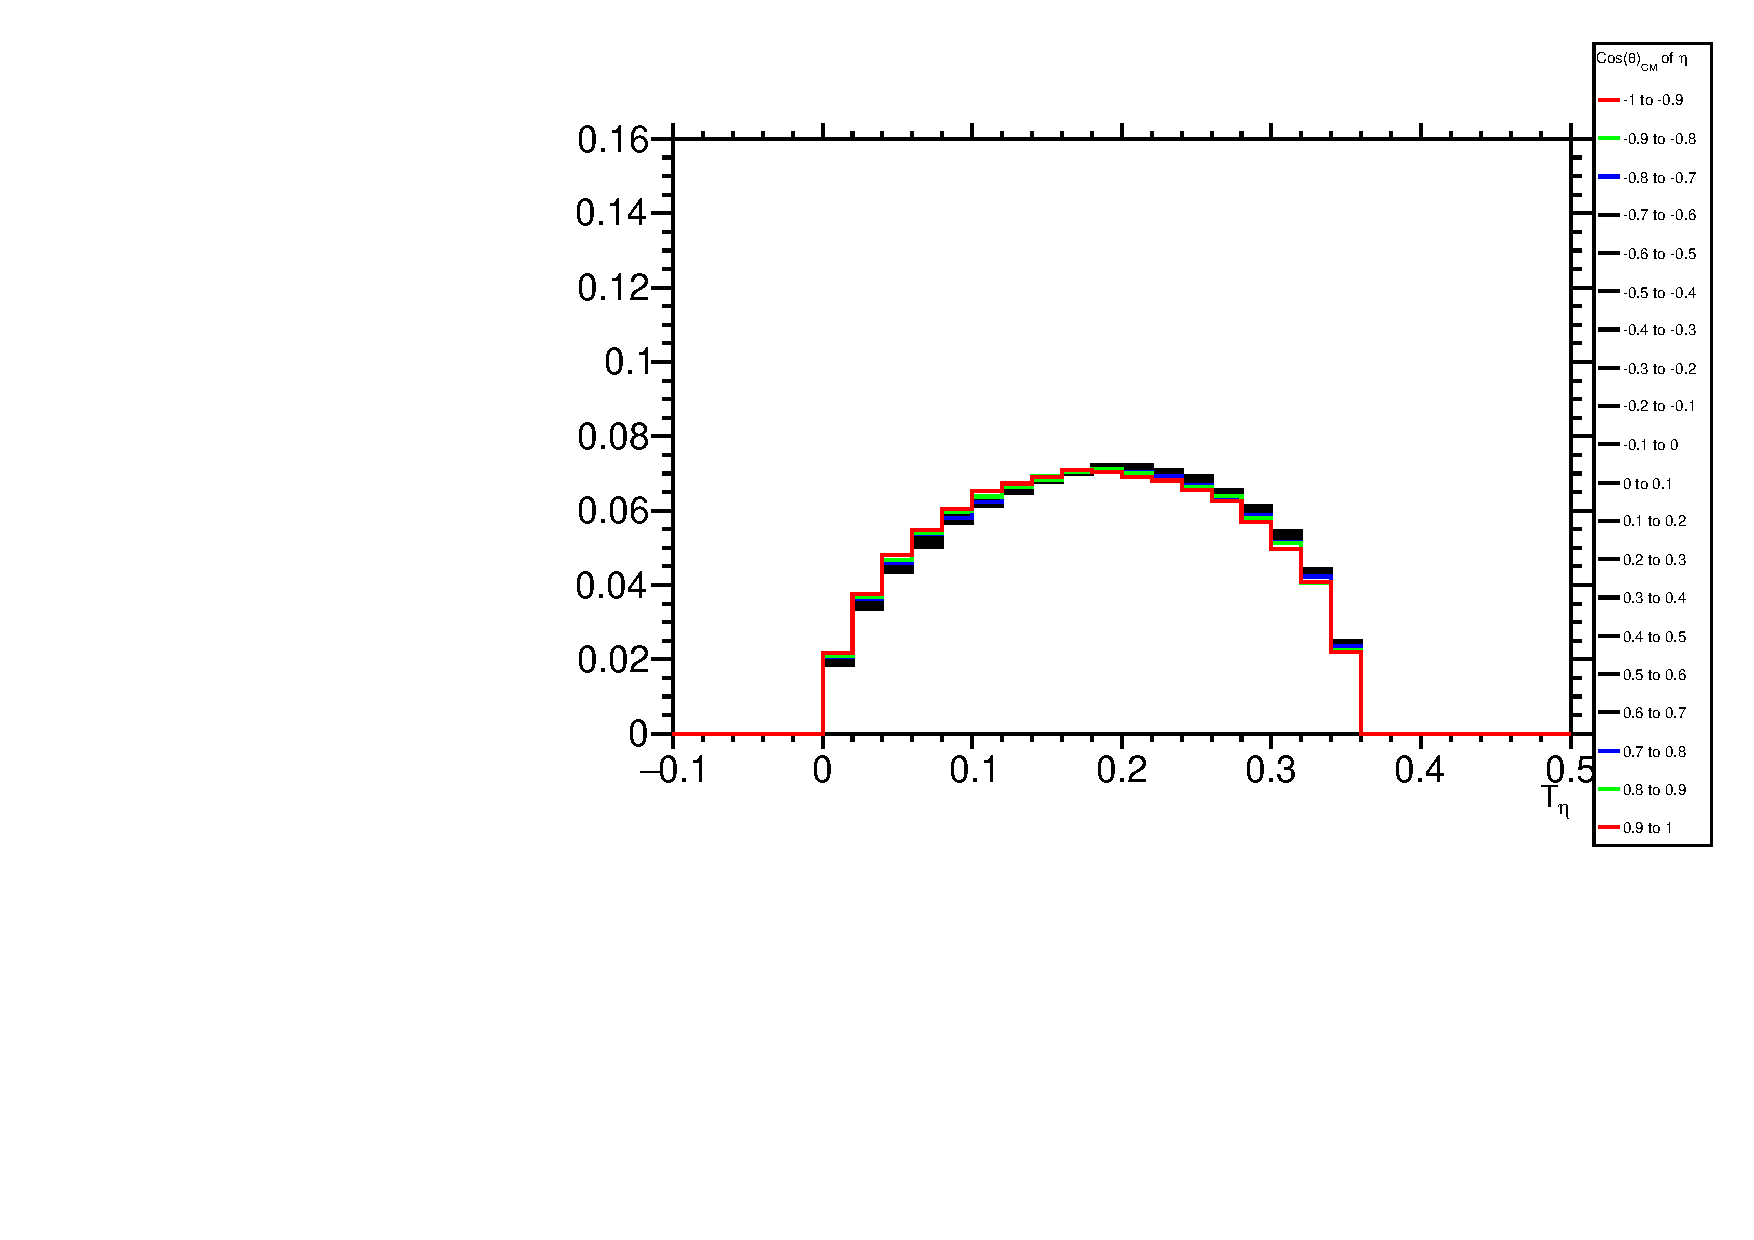
\includegraphics[width=12cm,height=8cm]{Gen_T.pdf}}
%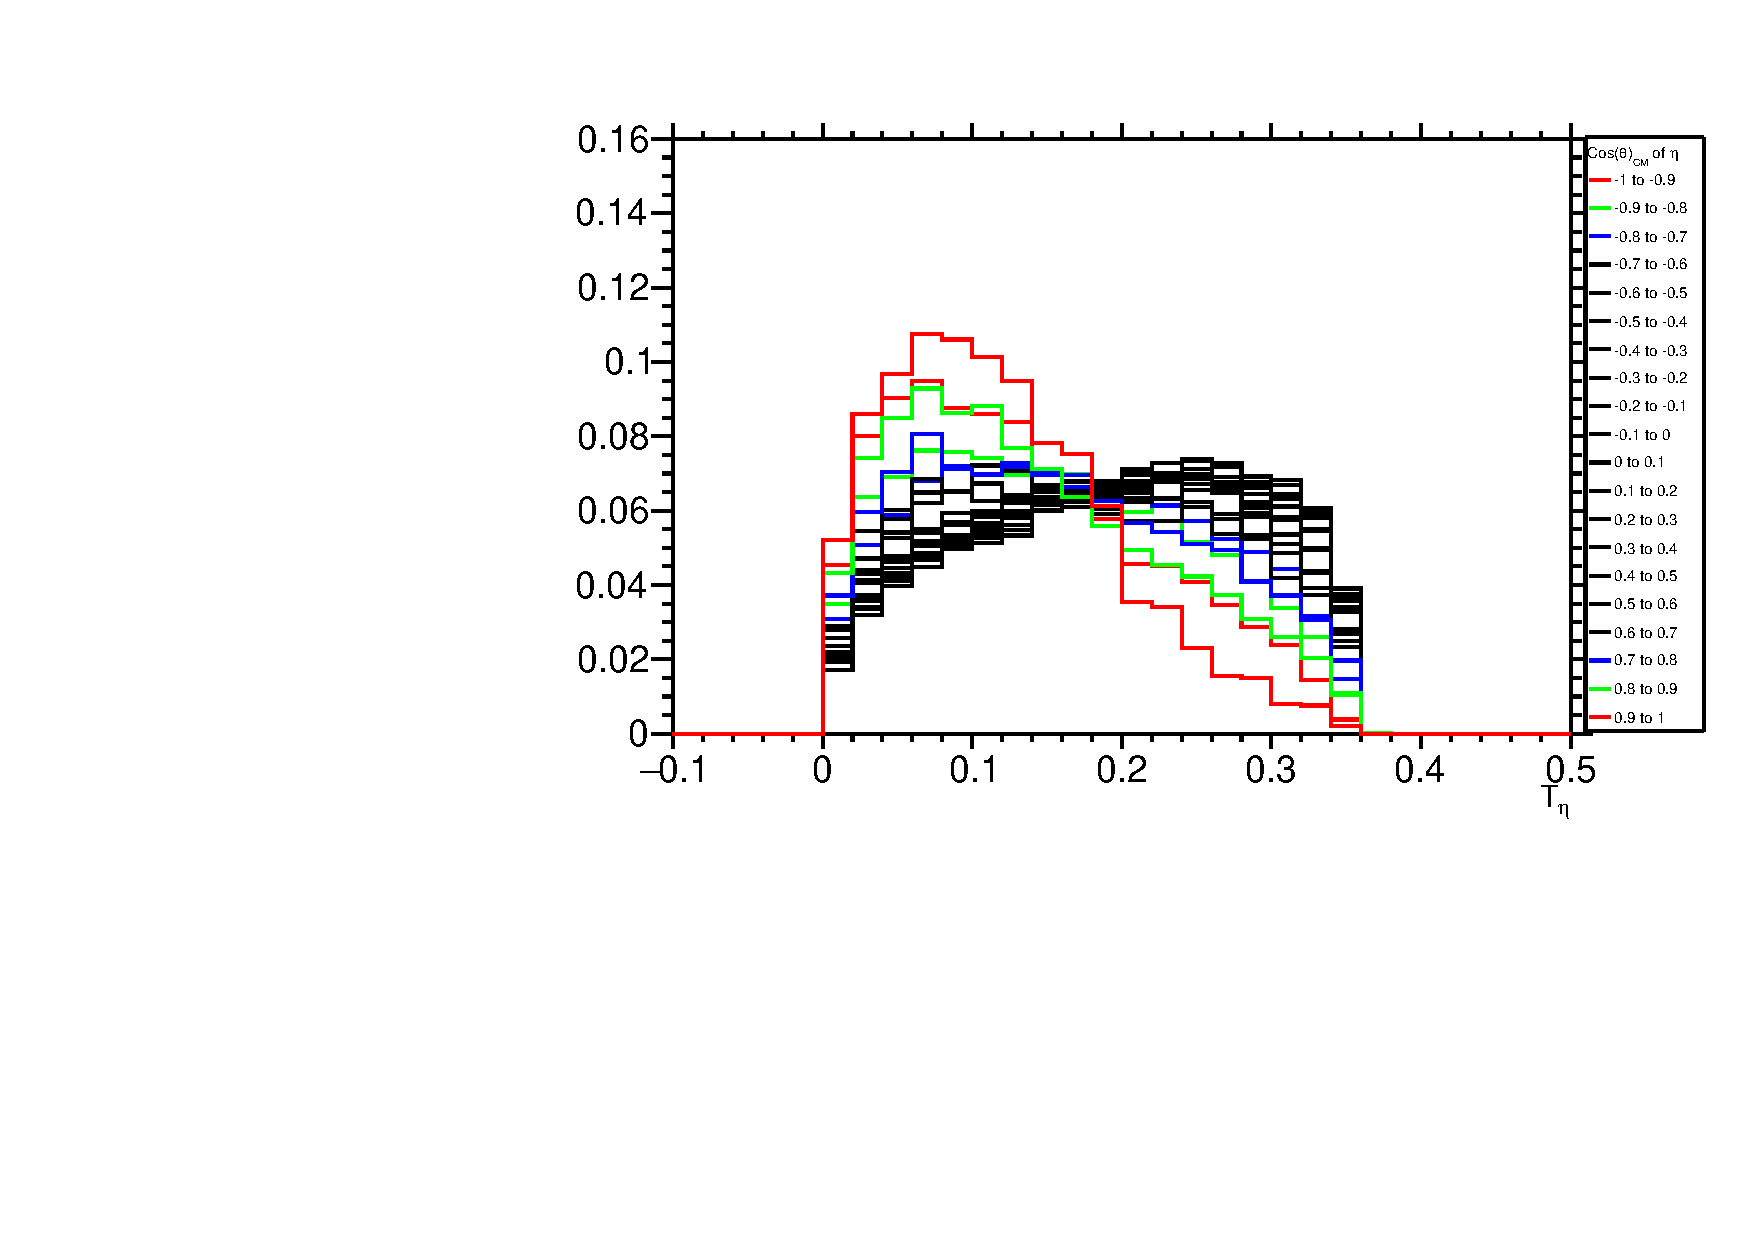
\includegraphics[width=12cm,height=8cm]{Sim_T.pdf}}
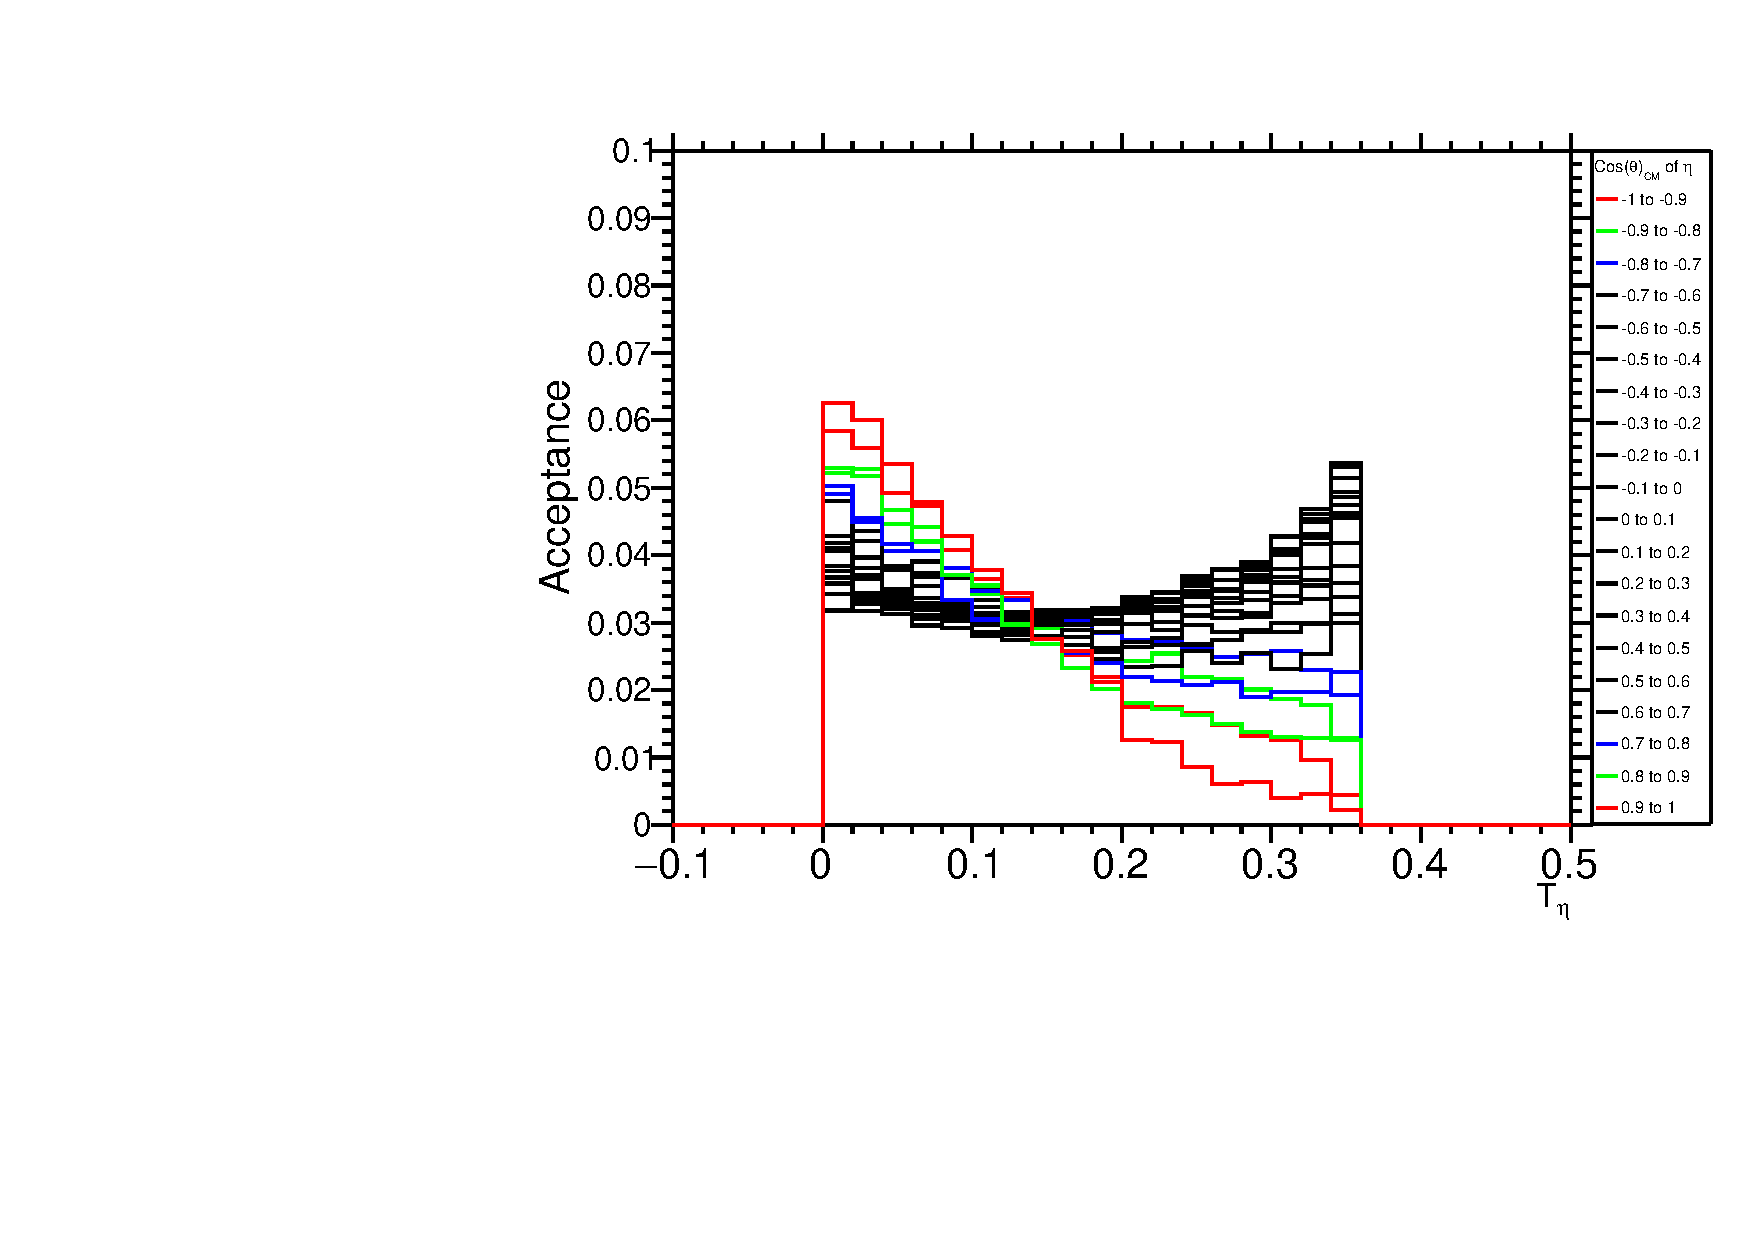
\includegraphics[width=12cm,height=8cm]{Acc_T.pdf}}
\caption{The acceptance vs $T_{\eta}$ in 0.1 bins of $\cos$ 
$\theta_{center-of-mass}$ of $\eta$ meson. }
\label{Fig_CsE_2}
\end{figure}

The kinematics of $\eta$ meson is directly related to the Dalitz variable Y. Hence a comparison of the cut is also presented for the Dalitz variable Y in Figure.~\ref{Fig_CsE_3} and  ~\ref{Fig_CsE_4} from simulation and g12 data respectively.    

\begin{figure}[ht!]
\centerline{
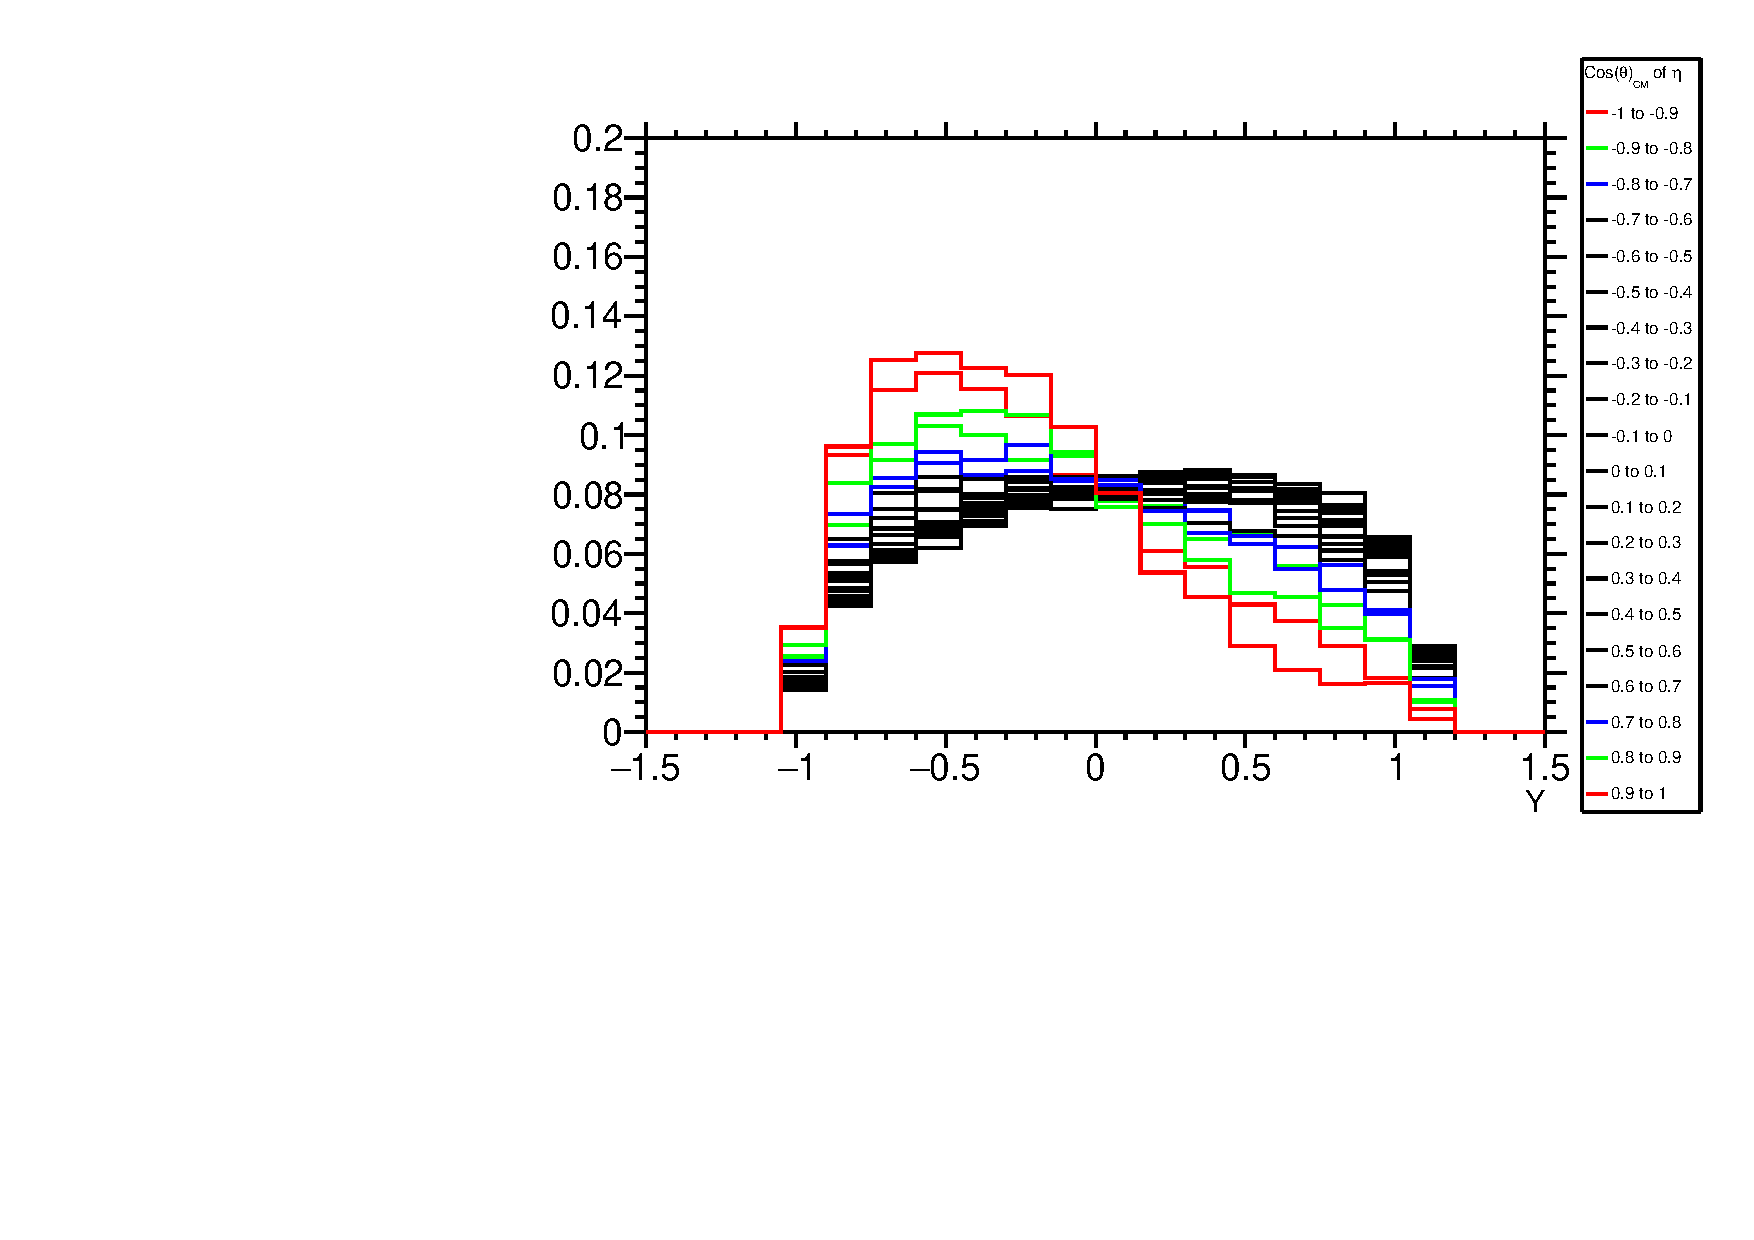
\includegraphics[width=12cm,height=8cm]{eta_CosTh_Cut.pdf}}
\caption{Dalitz Variable Y distribution normalised to 1 in each 0.1 bins of $\cos\theta_{center-of-mass}$ of $\eta$ from simulation.}
\label{Fig_CsE_3}
\end{figure}

\begin{figure}[ht!]
\centerline{
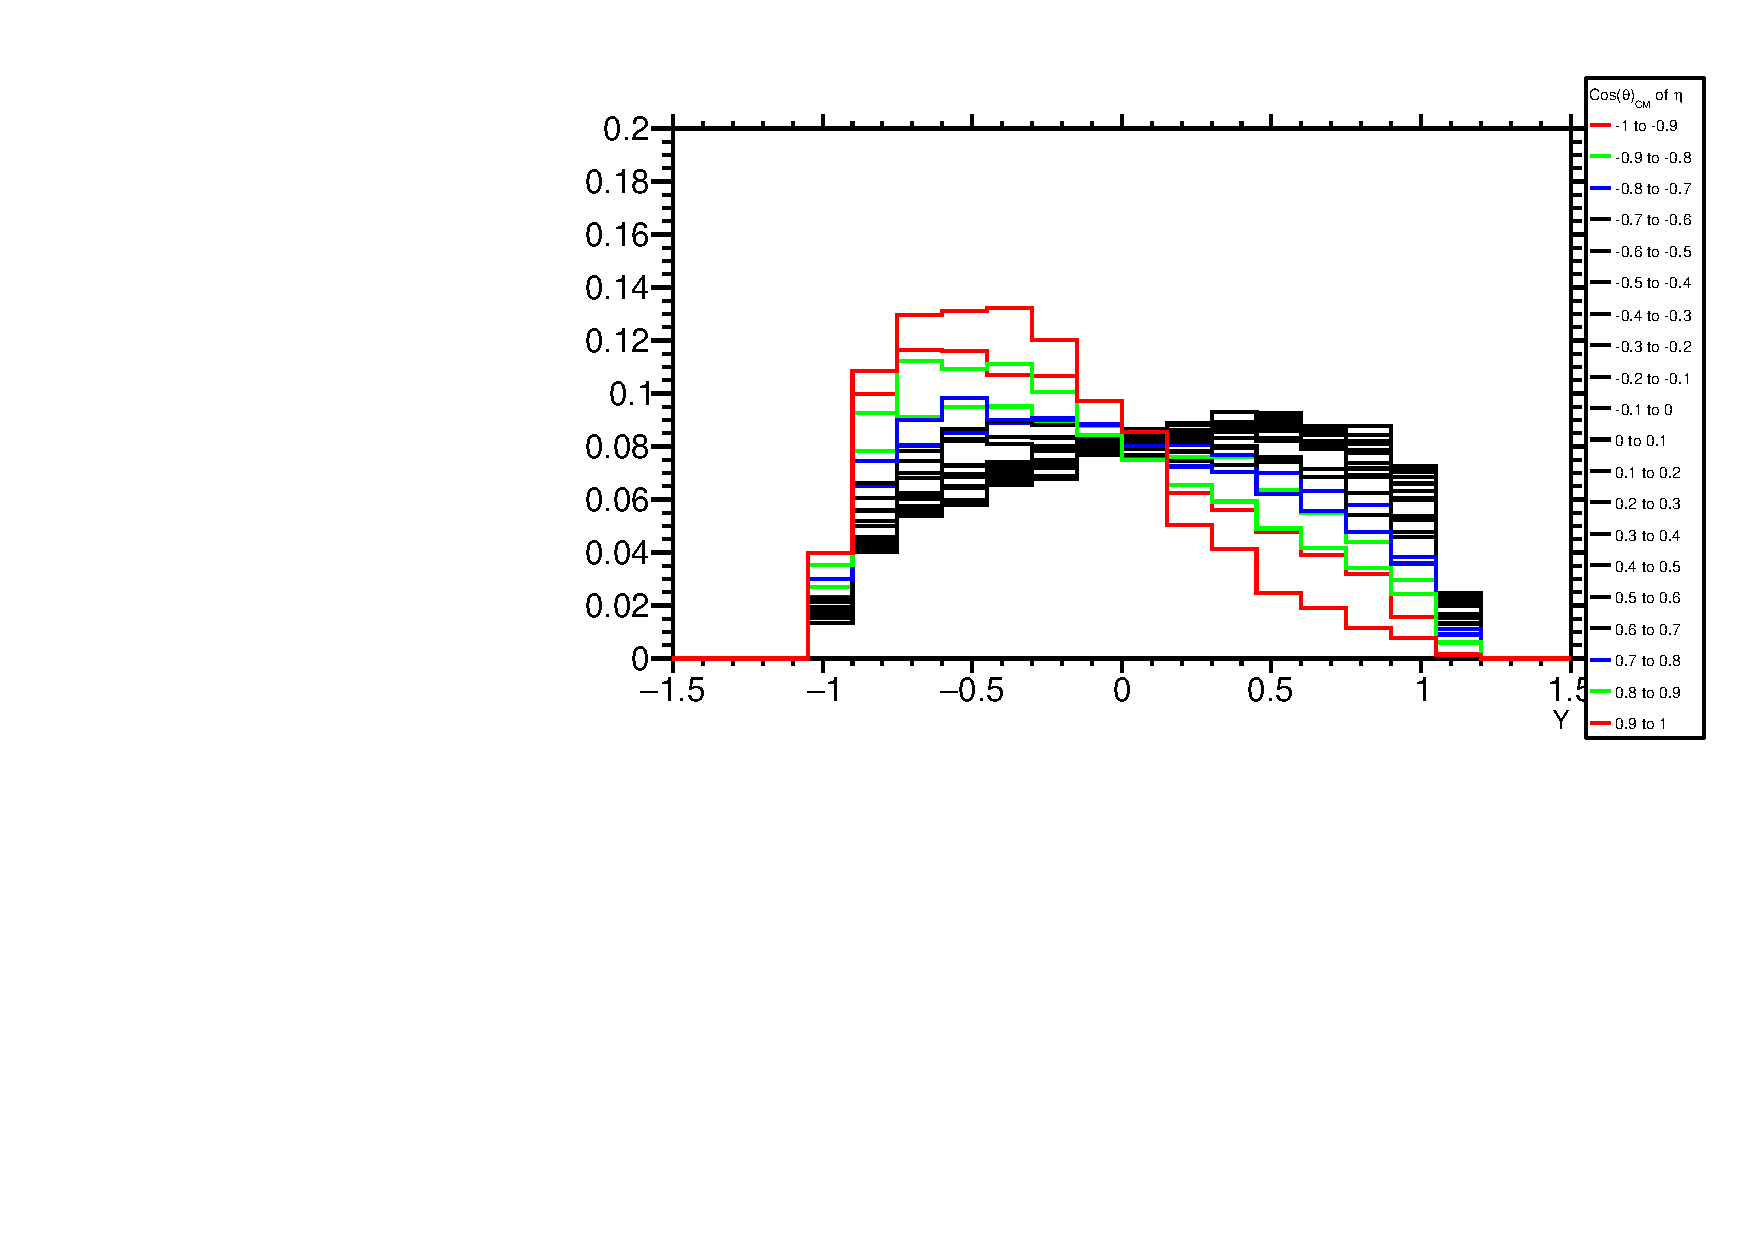
\includegraphics[width=12cm,height=8cm]{sim_CsEta.pdf}}
\caption{Dalitz Variable Y distribution normalised to 1 in each 0.1 bins of $\cos\theta_{center-of-mass}$ of $\eta$ from g12 data.}
\label{Fig_CsE_4}
\end{figure}

\subsection{Vetex Cut}
\label{VCut}
In the g12 experiment the target was positioned -90 cm from the CLAS center. The target cell was 40 cm long and 2 cm in radius in the form of a cylinder filled with unpolarised liquid hydrogen. We used this target information and imposed it to all event vertexes. We required all events  production vertex tracks to originate in the target region via the condition that $\sqrt{v_{x}^{2} + v_{y}^{2}}$ $\leq$ 2 cm and -110 $\geq$ $v_{z}$ $\leq$ -70 cm. 

\begin{figure}[ht!]
\centerline{
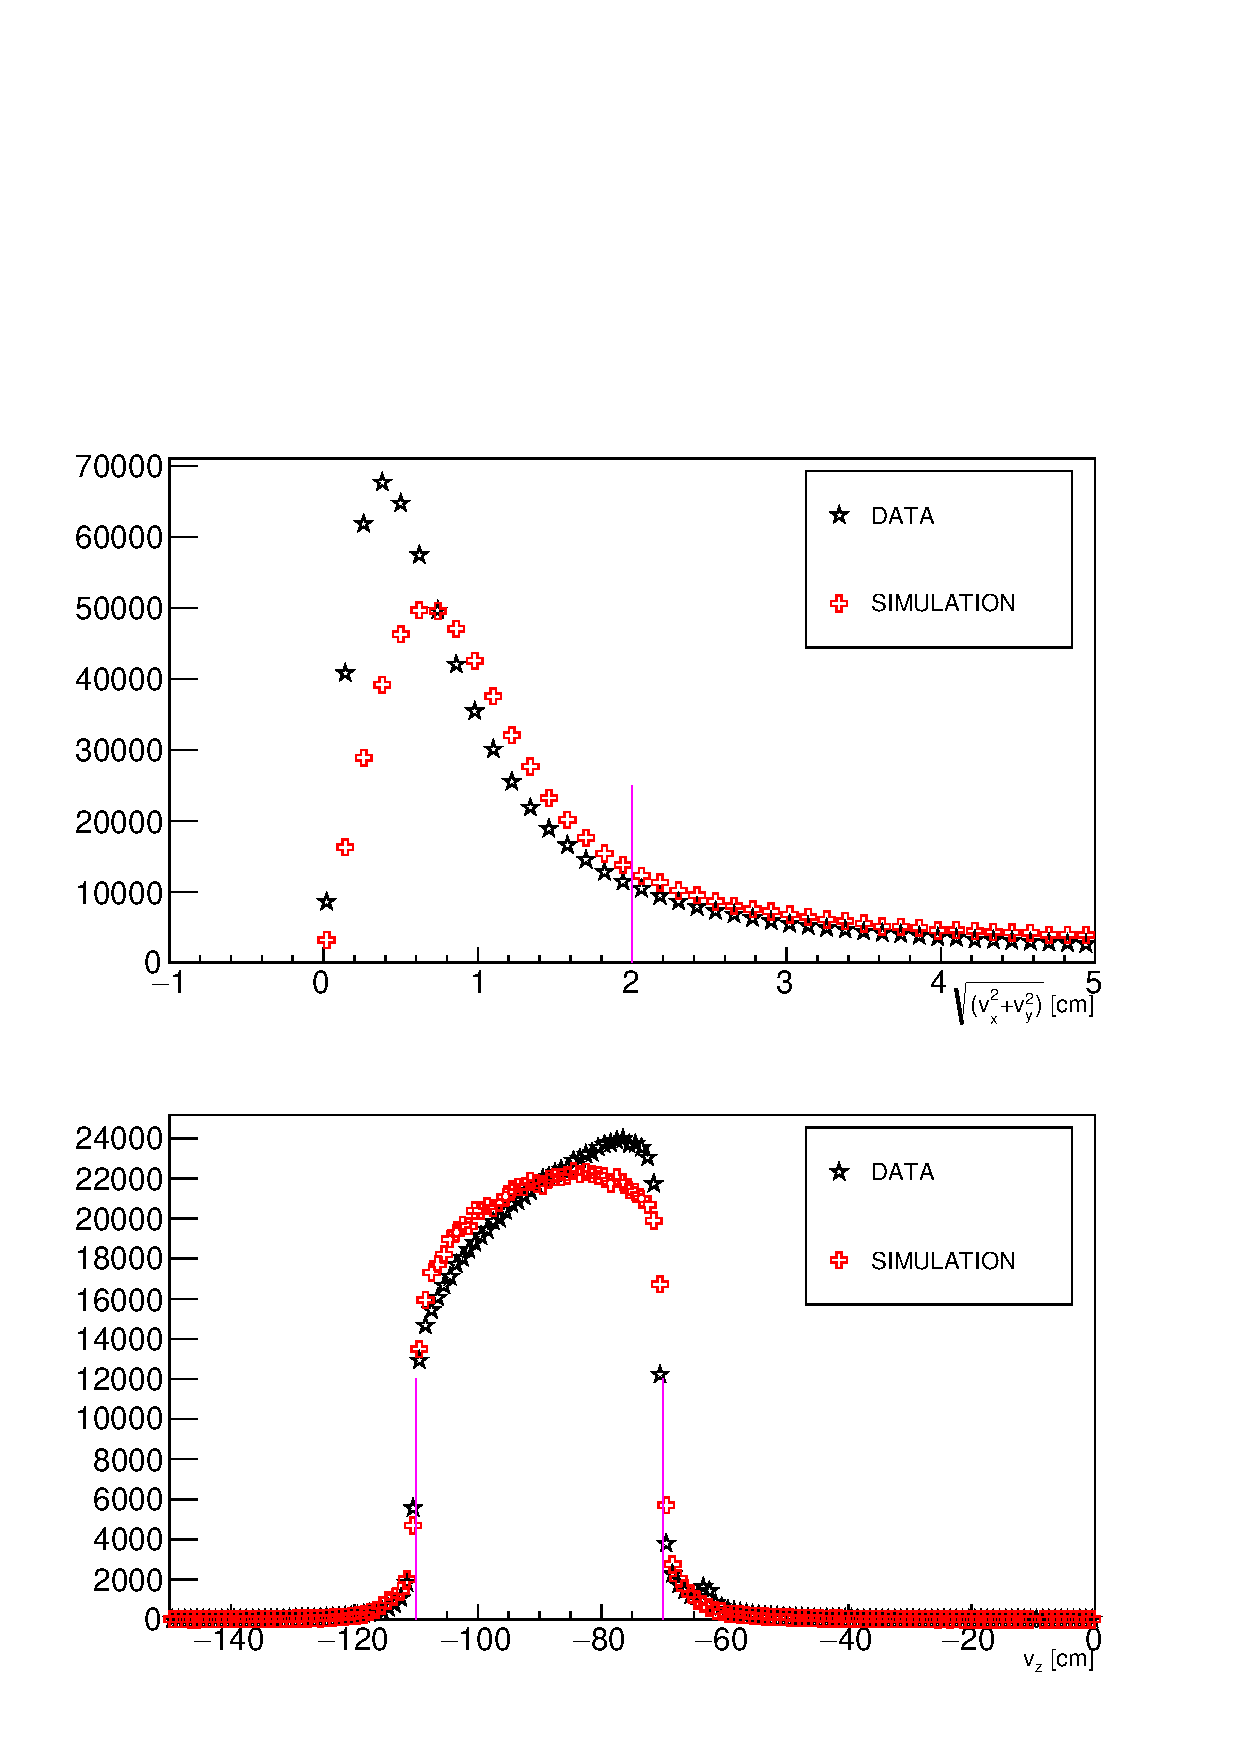
\includegraphics[height=5.8in]{vertex.pdf}}
\caption{[tpho + tprop -scvt] distribution from the simulation and data for proton, $\pi^{+}$ and $\pi^{-}$.}
\label{Fig1}
\end{figure}

\subsection{Timing Cuts on proton, $\pi^{+}$ and $\pi^{-}$}
\label{TCut}
As a post PID improvement of the detected final state particles $\pi^{+}$, $\pi^{-}$ and proton, we introduced a vertex timing $(t_{vert})$ cut of particles in the analysis. The $t_{vert}$, vertex time is the instant of time the particle left the target. One can calculate it through the information of the TOF detectors as,

\begin{eqnarray*}
t_{vert}(TOF) = t_{TOF}  -  \frac{l_{TOF}}{c\beta}
\end{eqnarray*}

where $t_{TOF}$ and $l_{TOF}$ are the measured time and length of particle in TOF sub detector. Here c is the velocity of light in vacuum and $\beta$ is the Lorentz factor of the particle calculated by knowing the velocity(v) of particle as $\beta = \frac{v}{c}$. The same vertex timing $(t_{vert})$ information can also be calculated from the RF-corrected time instant of the photon ($t_{photon}$)  crossing the target center measure by the tagger added with the $t_{prop}$, which is the propagation time from the center of the target to the track vertex. Given by,

\begin{eqnarray*}
t_{vert}(Tagger) = t_{photon} + t_{prop}.
\end{eqnarray*}


The difference of the $t_{vert}(TOF)$ from $t_{vert}(Tagger)$ is shown in Fig.$~\ref{Fig2}$, and we make a cut of $\pm$ 1.55 ns around 0 ns for all the final state particles in both simulation and data. 
\begin{figure}[ht!]
\centerline{
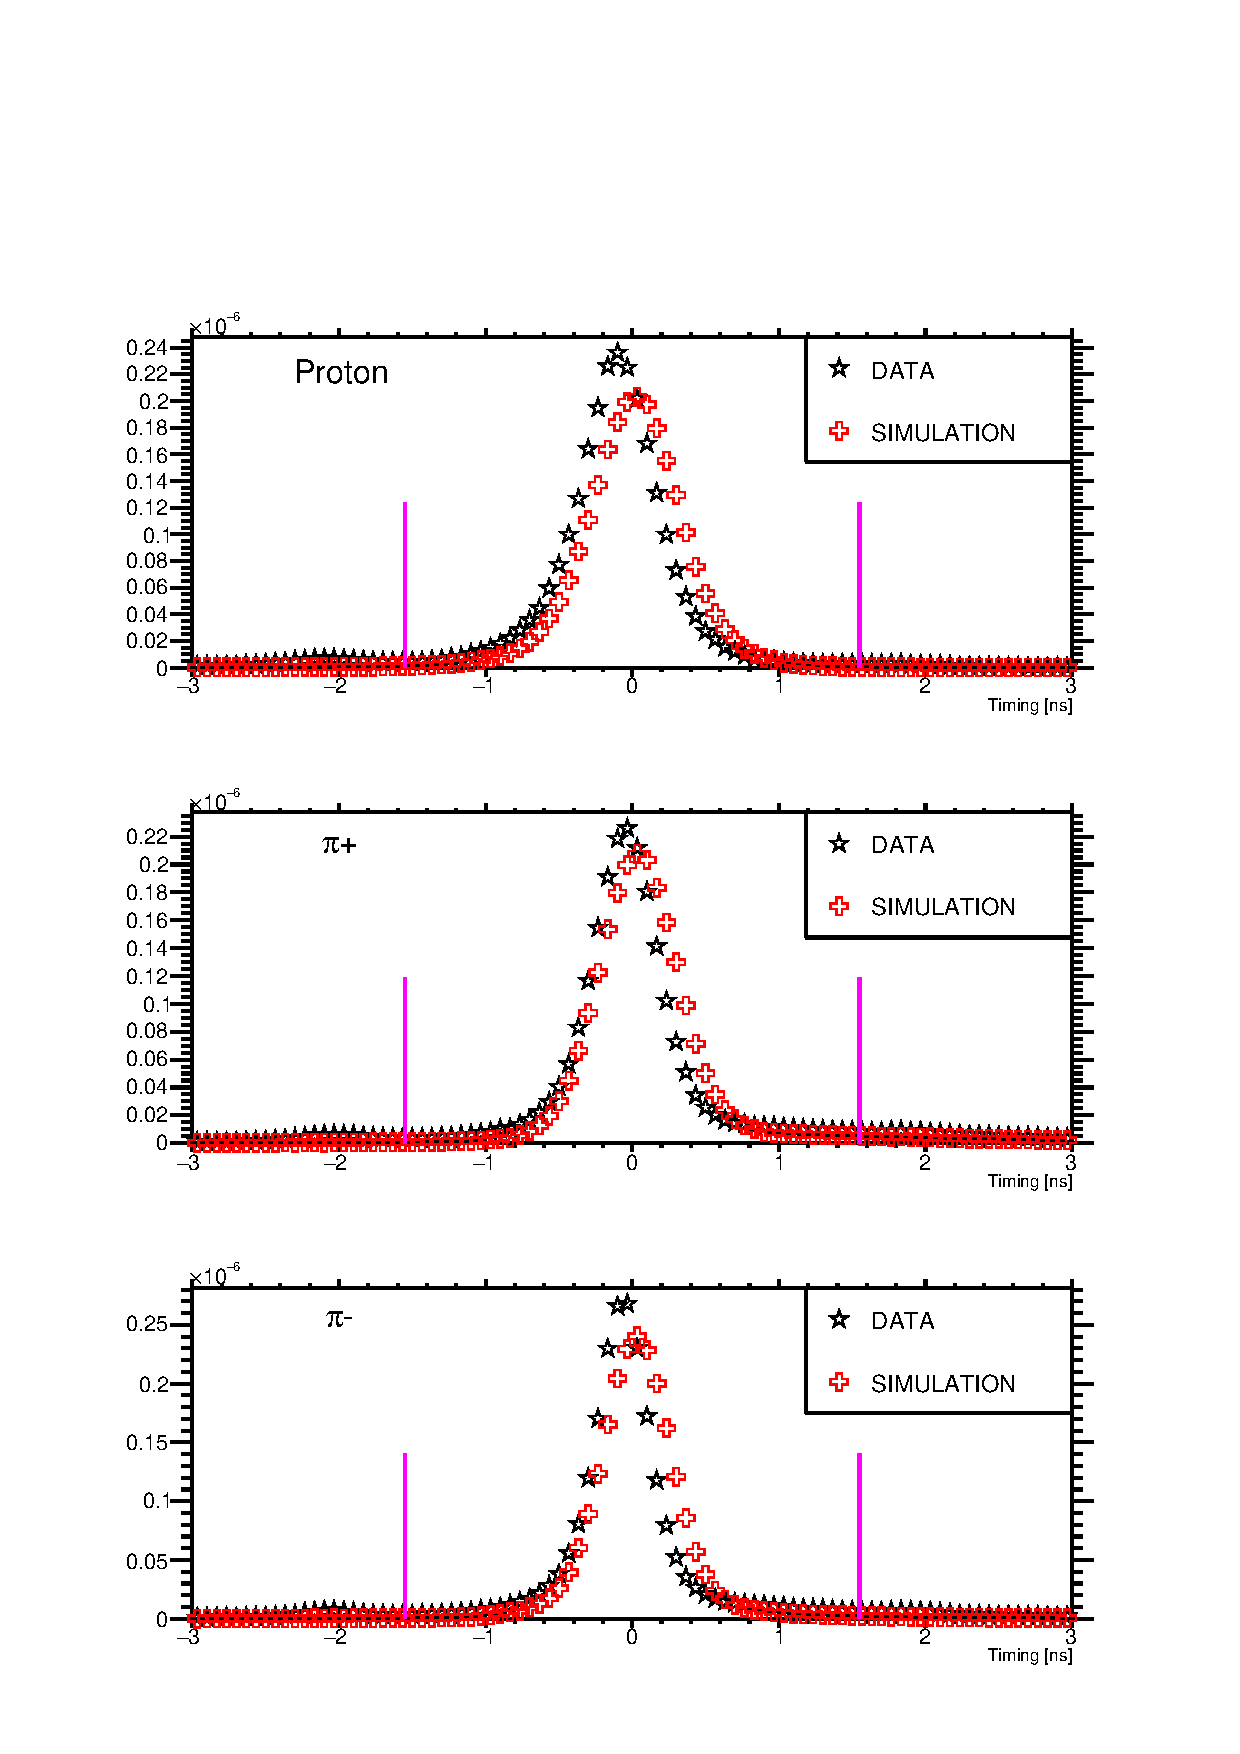
\includegraphics[height=7.8in]{timing.pdf}}
\caption{[$t_{vert}(TOF)$ - $t_{vert}(Tagger)$] distribution from the simulation and data for proton(Upper), $\pi^{+}$(Middle) and $\pi^{-}$(Lower).}
\label{Fig2}
\end{figure}

\section{Result}

The simulated events and g12 data are passed all selection and cuts described in  Section.~\ref{Cor}, Section.~\ref{VCut}, Section.~\ref{TCut}, Section.~\ref{Cos} and Section.~\ref{KF}. The number of the events rejected in both the simulation and data after the cuts is shown in a Table.~\ref{tab3}. 
  
\begin{table}[]
\centering
\begin{tabular}{|c|c|c|}
\hline
Cuts                                        & g12 Run 56655                    & Simulation \\
\hline
Generated                               & ---                          & 10001500   \\
Reconstructed                           & 42947                        & 855447     \\
Vertex Cut                              & 20092                        & 505405     \\
Timing Cut                              & 11390                        & 451470     \\
Multiple $E_{\gamma}$ & 14986 & ---            \\
Fiducial Cuts                           & 10541                        & 276432     \\
Prob(($\eta$)$\pi^{+}$$\pi^{-}$p) \textgreater 0.01                & 1901                         & 259136    \\
\hline
\end{tabular}
\caption{The table shows the cut flow of the analysis from g12 data run 56655 and simulated events.}
\label{tab3}
\end{table}
 
 In an attempt to see how well the simulation explains the g12 data a comparison of the kinematic variables of the center-of-mass energy ($\sqrt{s}$) and momentum (P), $\theta$ and $\phi$ for $\pi^{+}$ $\pi^{-}$ and p is shown in the Figure.~\ref{fig6}, ~\ref{fig7}, ~\ref{fig8} $\&$ ~\ref{fig9}. The events in the Monte Carlo are generated with the model explained in Section.~\ref{Sim} with the input Dalitz plot parameters from BESIII measurement~\cite{Ablikim:2010kp}.

\begin{figure}[ht!]
\centerline{
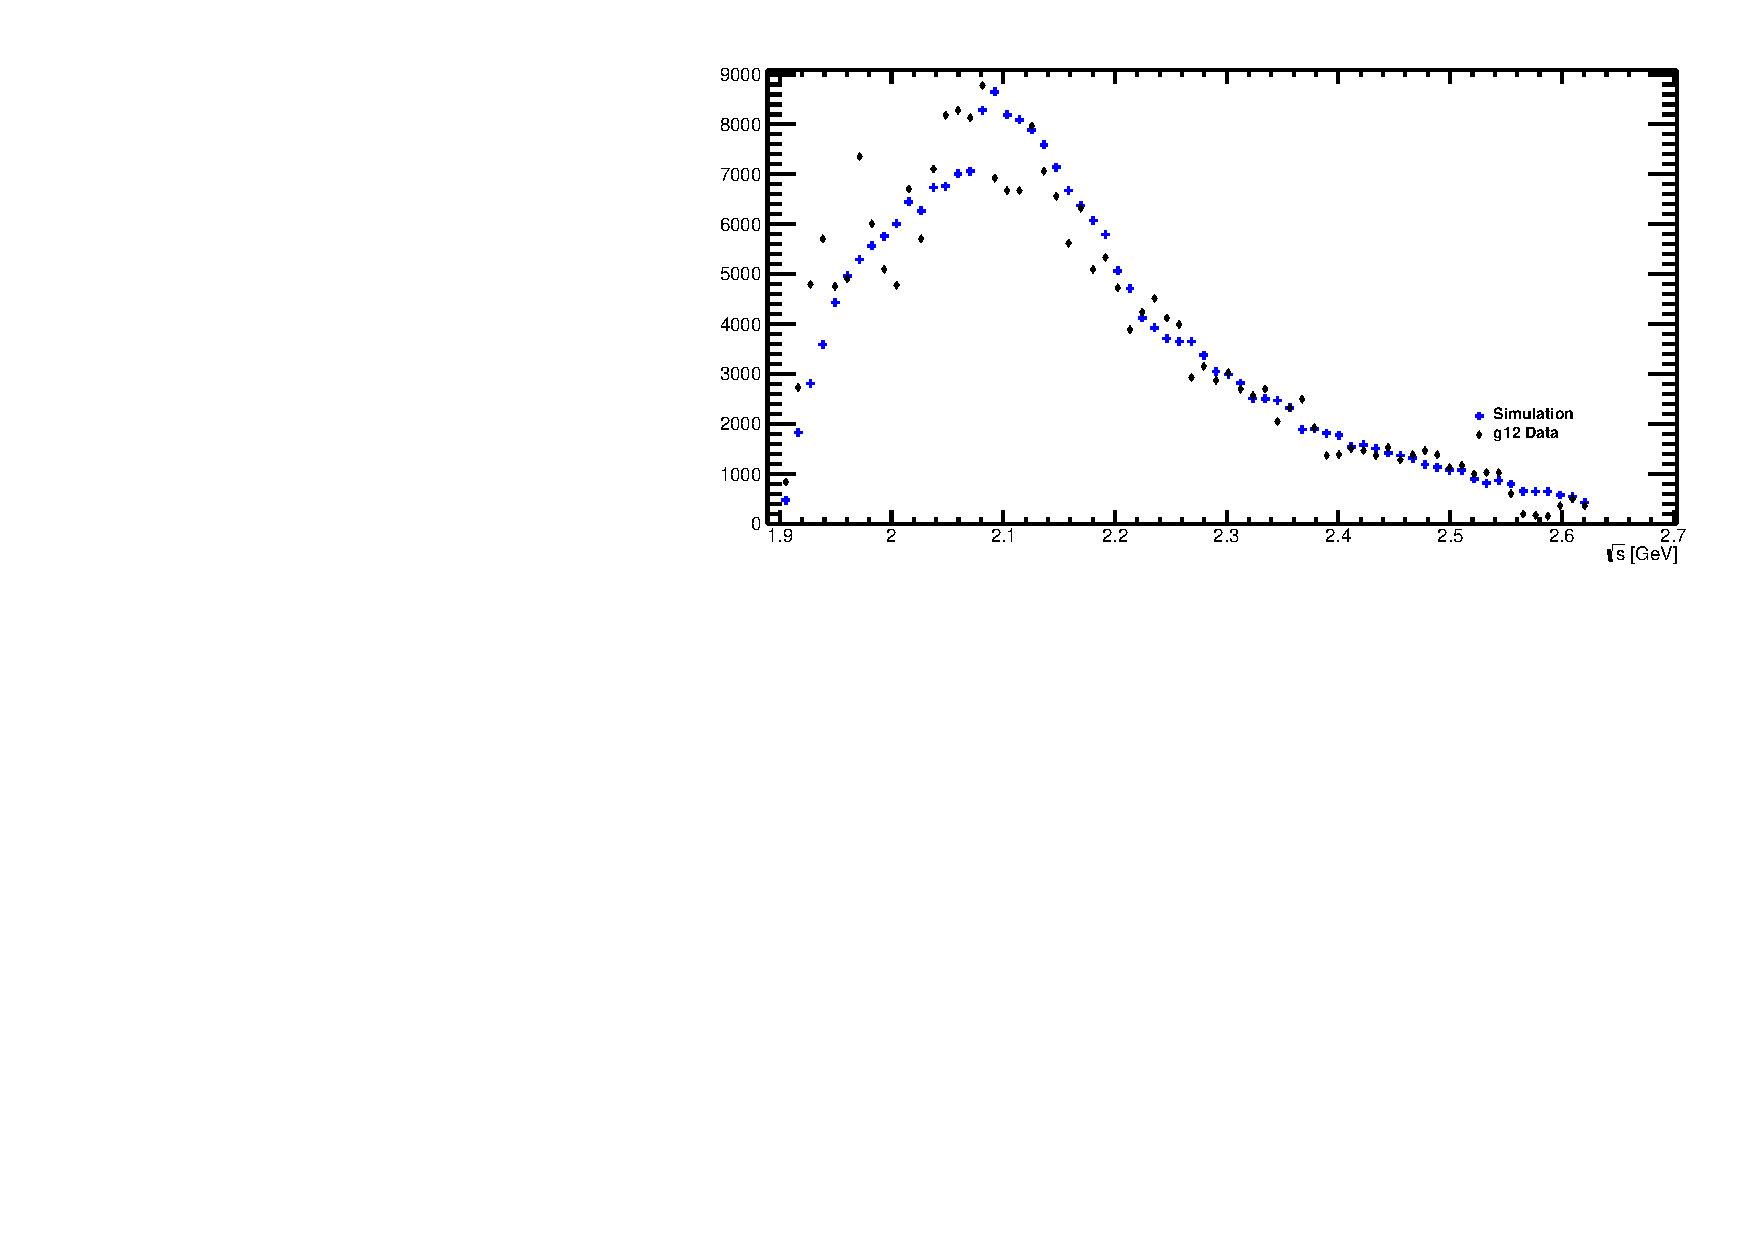
\includegraphics[width=10cm,height=6cm]{w.pdf}}
\caption{Comparison of incident photon beam in center of mass energy ($\sqrt{s}$) with simulated (blue) events and g12 data (black) when generating Monte-Carlo with the differential cross-sections and Dalitz plot parameters.}
\label{fig6}
\end{figure}

\begin{figure}[ht!]
\centerline{
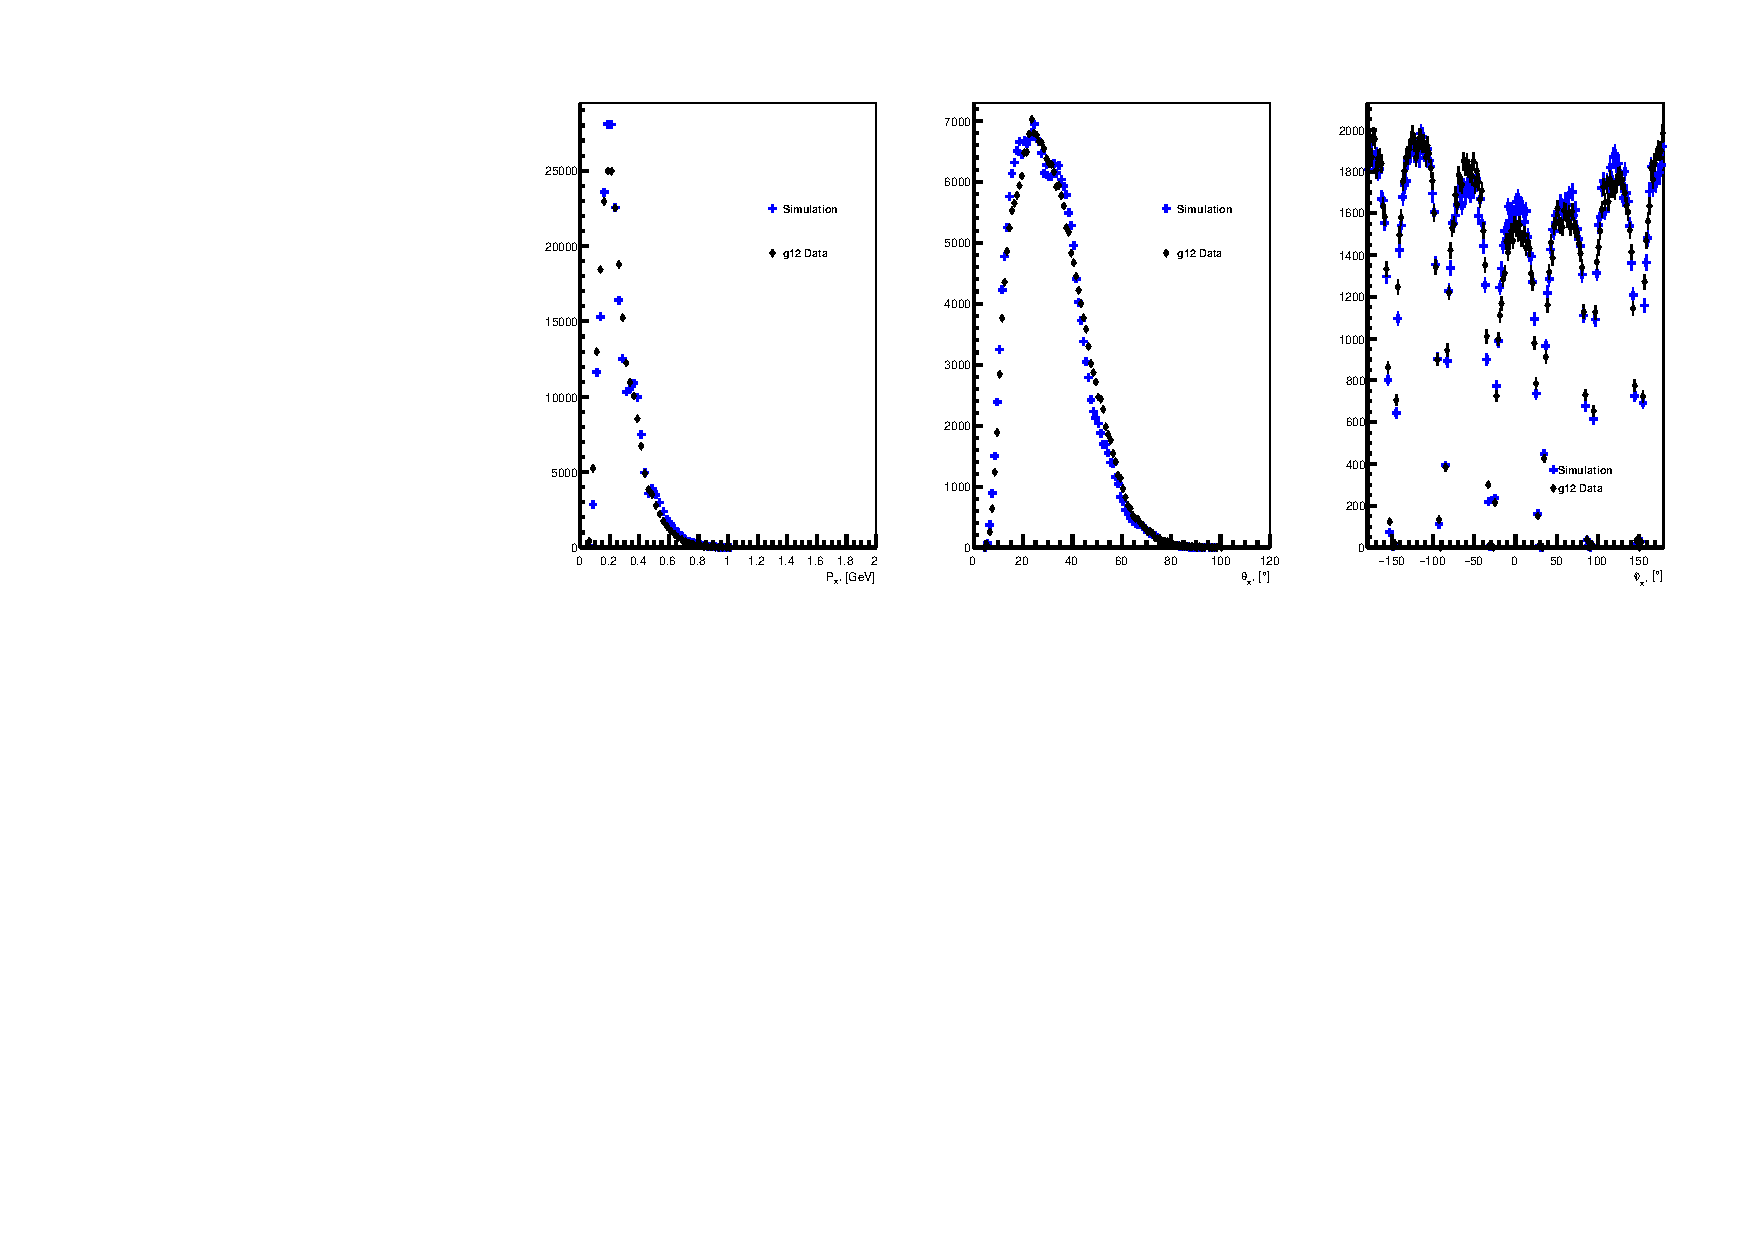
\includegraphics[width=14cm,height=4cm]{Pip.pdf}}
\caption{Comparison of  $\pi^{+}$ momentum (left), $\pi^{+}$ $\theta$ (middle) and $\pi^{+}$ $\phi$ (right) with simulated (blue) events and g12 data (black) when generating Monte-Carlo with the differential cross-sections and Dalitz plot parameters.}
\label{fig7}
\end{figure}
 
\begin{figure}[ht!]
\centerline{
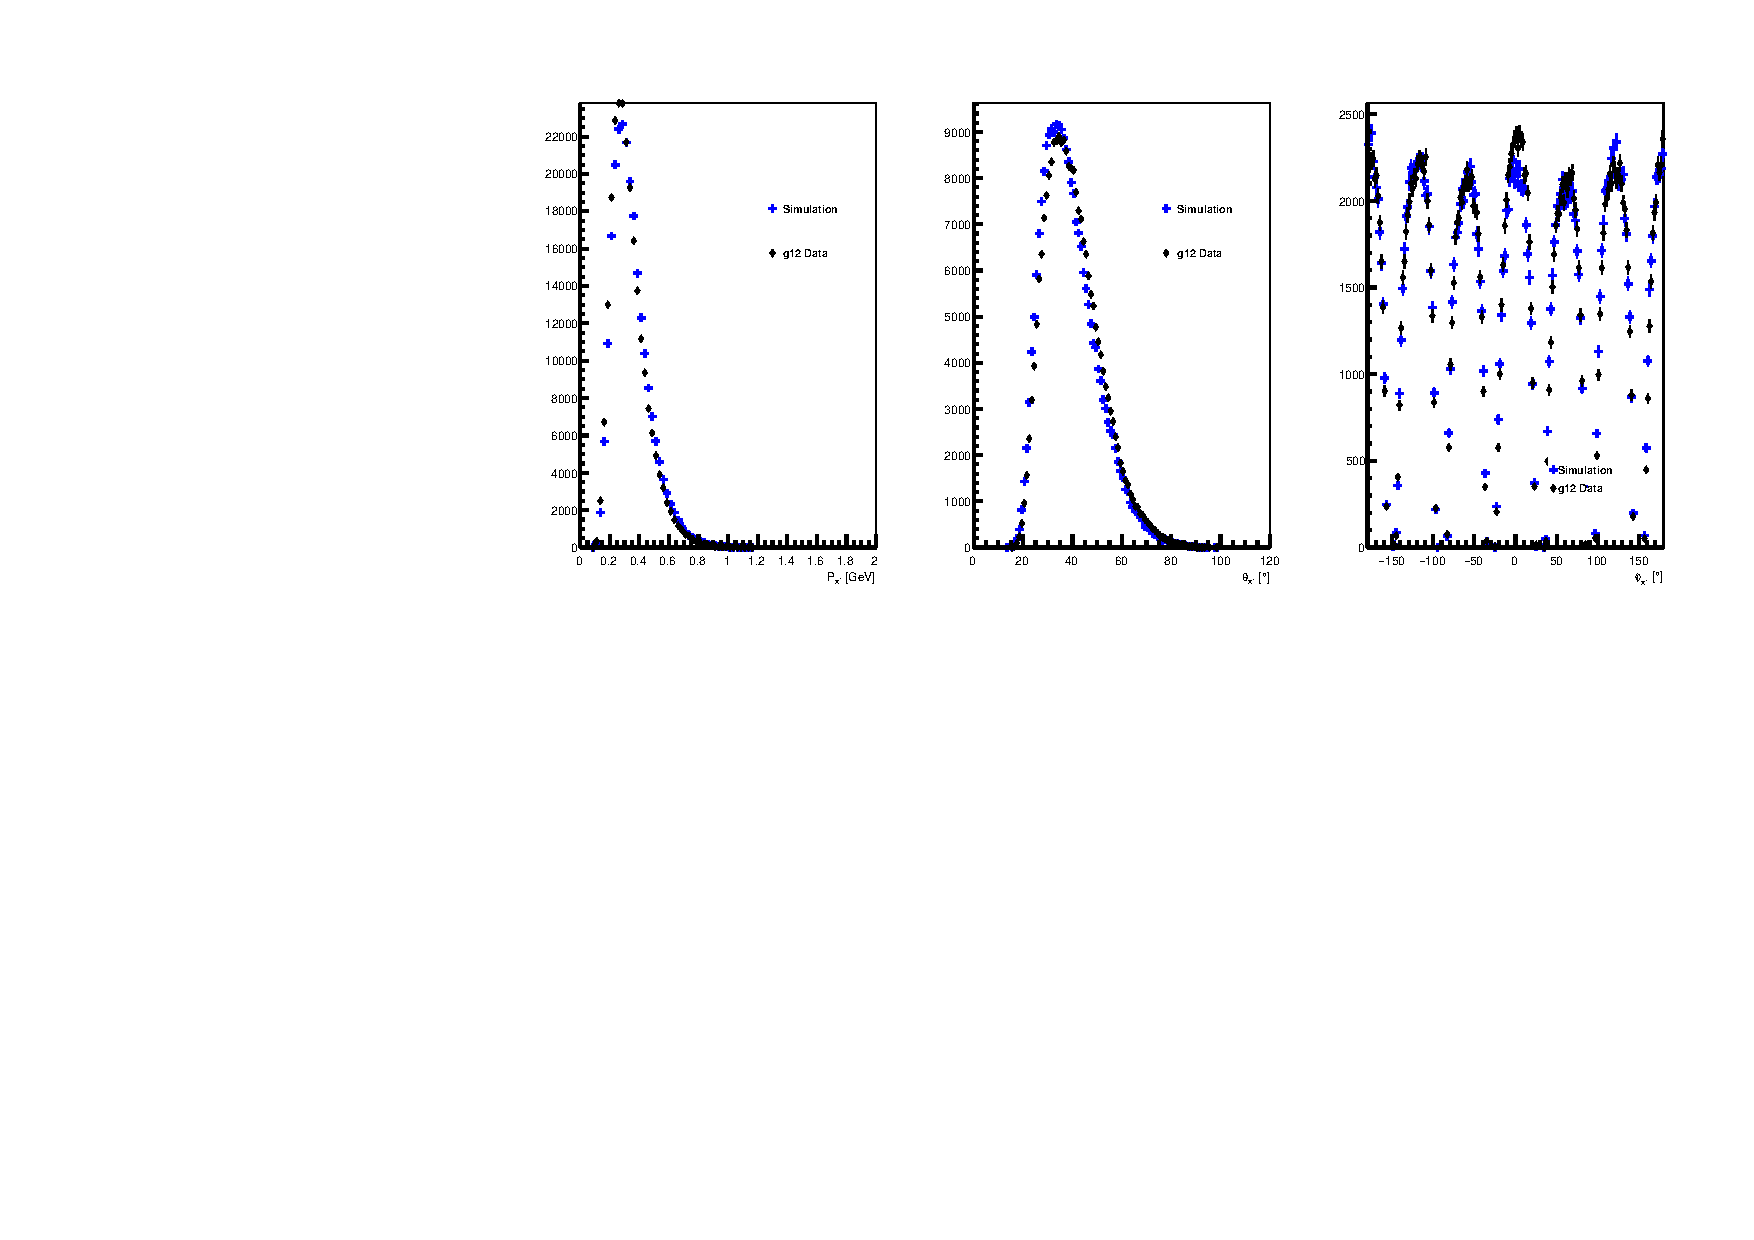
\includegraphics[width=14cm,height=4cm]{Pim.pdf}}
\caption{Comparison of $\pi^{-}$ momentum (left), $\pi^{-}$ $\theta$ (middle) and $\pi^{-}$ $\phi$ (right) with simulated (blue) events and g12 data (black) when generating Monte-Carlo with the differential cross-sections and Dalitz plot parameters.}
\label{fig8}
\end{figure}

\begin{figure}[ht!]
\centerline{
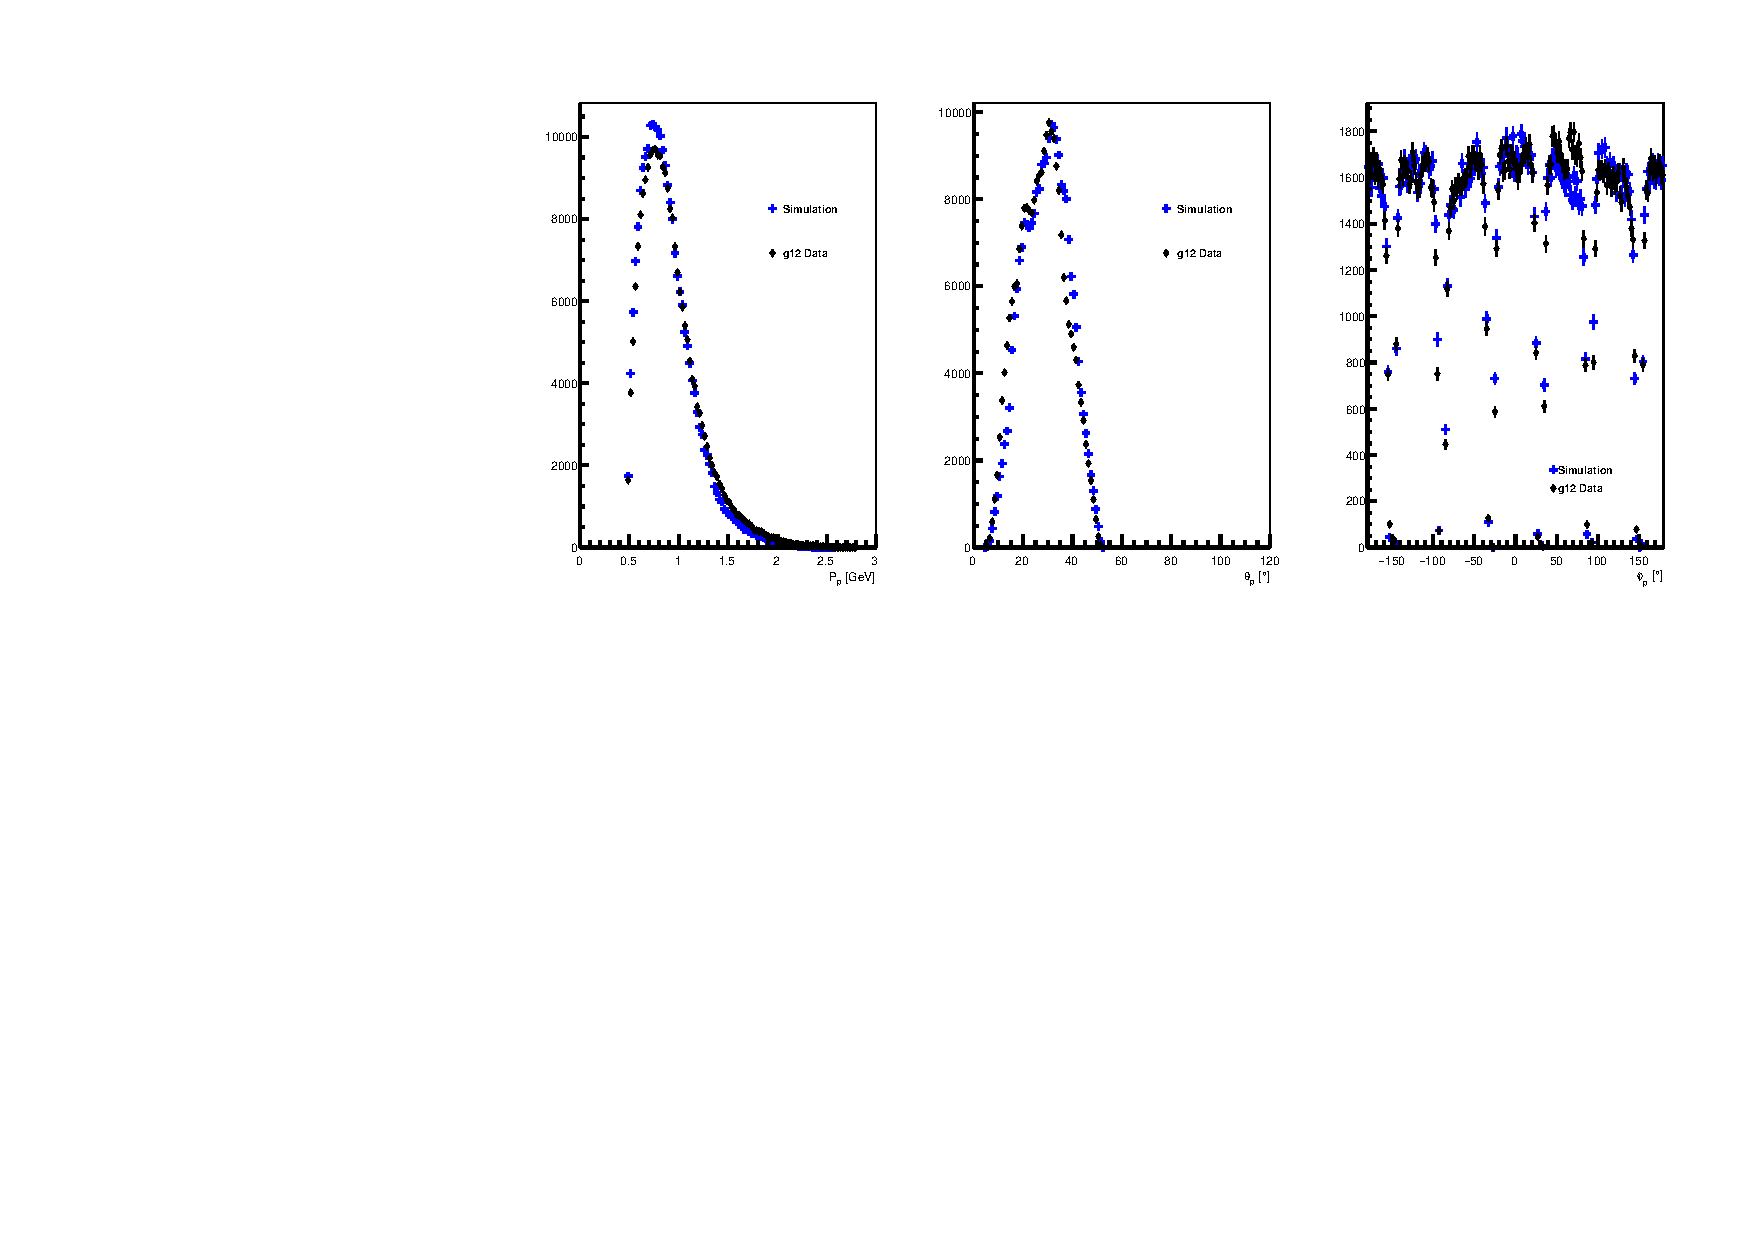
\includegraphics[width=14cm,height=4cm]{P.pdf}}
\caption{Comparison of proton momentum (left), proton $\theta$ (middle) and proton $\phi$ (right) with simulated (blue) events and g12 data (black) when generating Monte-Carlo with the differential cross-sections and Dalitz plot parameters.}
\label{fig9}
\end{figure}
 
 
 \subsection{Background subtraction to the Dalitz plot}

\begin{figure}[ht!]
\centerline{
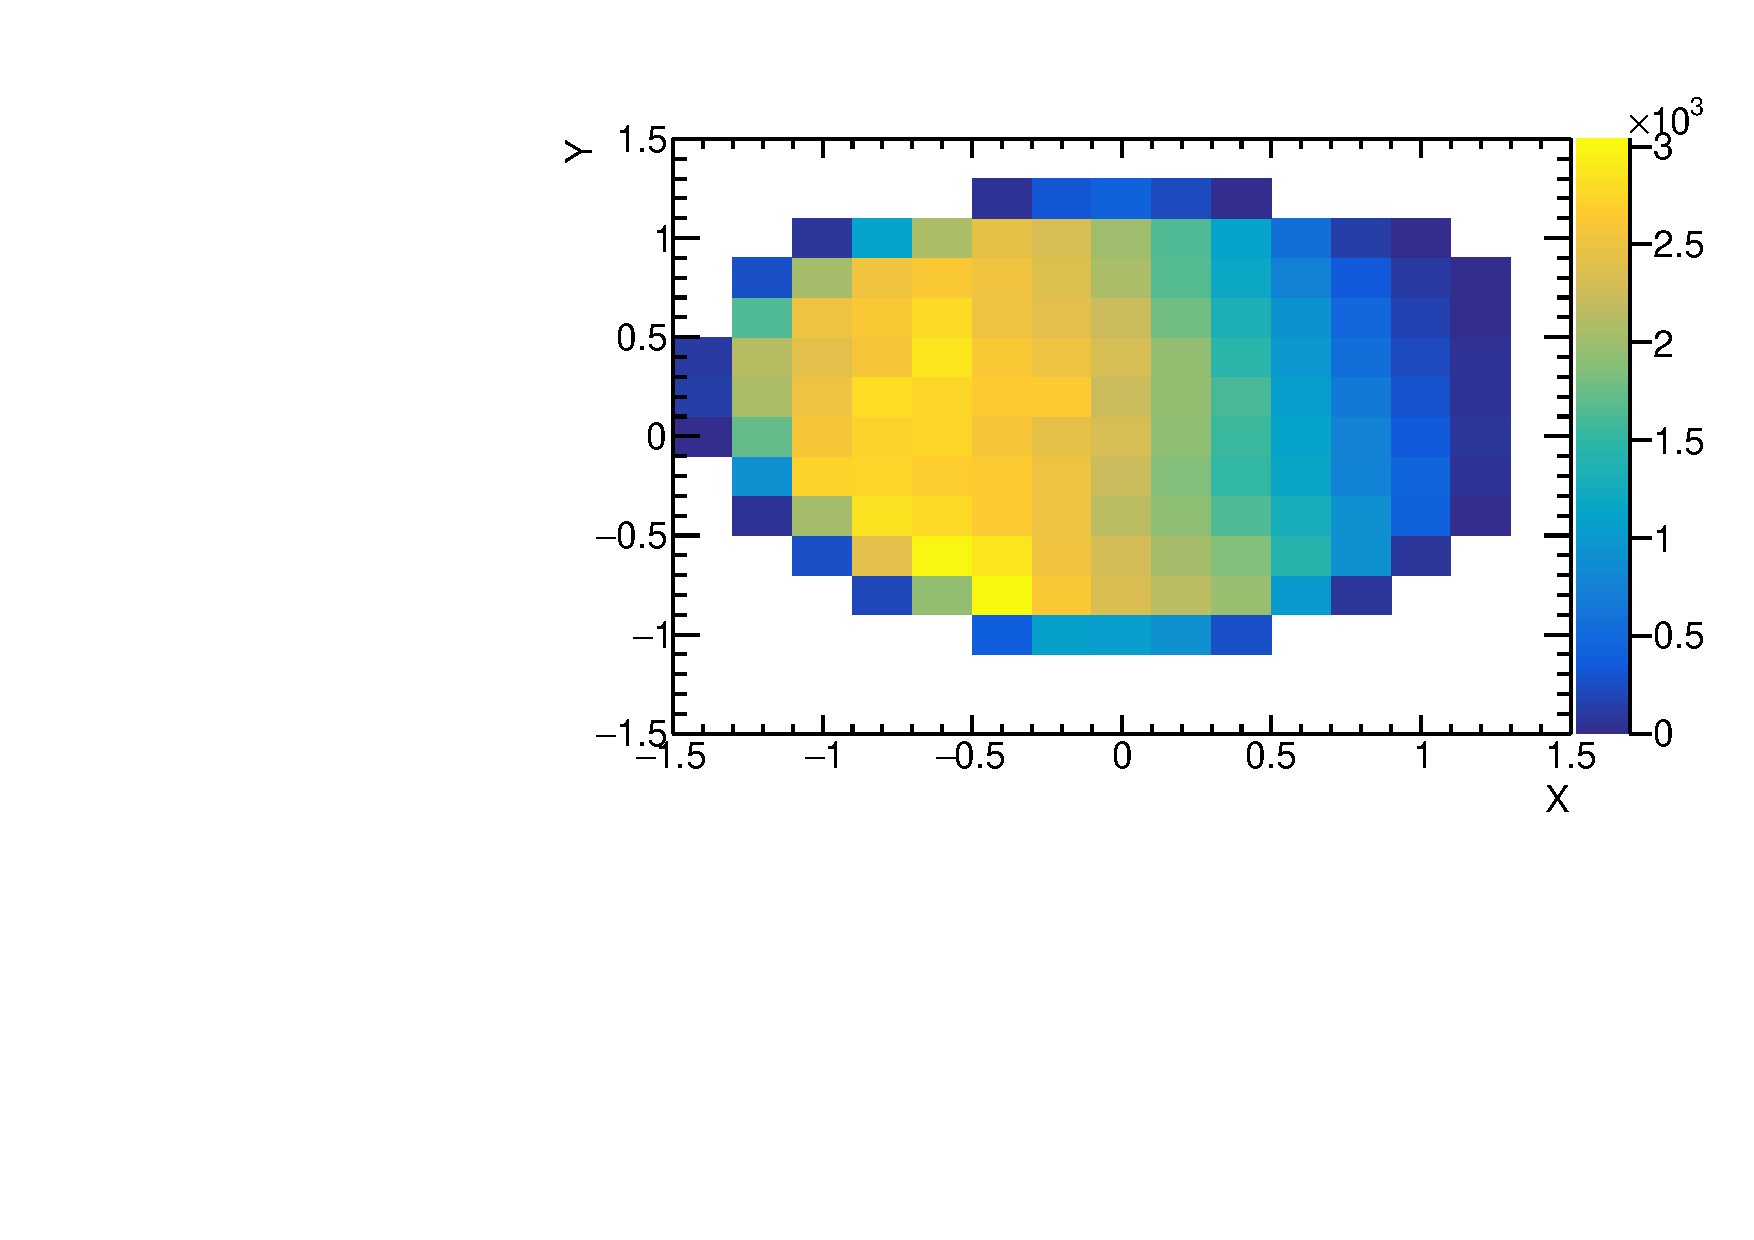
\includegraphics[width=10cm,height=6cm]{Before_BS.pdf}}
\caption{Dalitz plot before background subtraction.}
\label{B4_DP}
\end{figure}

The aim is to obtain a bin-wise background subtracted Dalitz plot. In order to achieve that all the events are feed into a X and Y (nbin x nbin) Dalitz plot and a bin-wise background subtraction is performed to the $M_{x}$(p) distribution after restricting 0.537 $\leq$ $M_{x}$(p$\pi{+}$$\pi{-}$) $\leq$ 0.557. The signal in $M_{x}$(p) distribution is fitted with a Voigt function and background is fitted with a Polynomial of order 3 in each bin of the Dalitz plot to subtract the non-resonant contribution. The fit to a low and high statistics bin shown in Figure.~\ref{DP_fit}. The events under the background subtracted 3 standard deviation region is the number of events in the Dalitz plot bin. The number of events in each Dalitz plot bin has ``$N_{i}$" events and the error is ``$\sigma_{i}$", given by 
\begin{equation}
\sigma = \sqrt{S_{1} + (S+B - S_{1})}
\end{equation}
where ``i" goes from 1 to total number of bins in the Dalitz plot. $S_{1}$ is the background subtracted peak and S+B is the total number of events in the $M_{x}$(p) spectrum in the 3 standard deviation.

\begin{figure}[ht!]
\centerline{
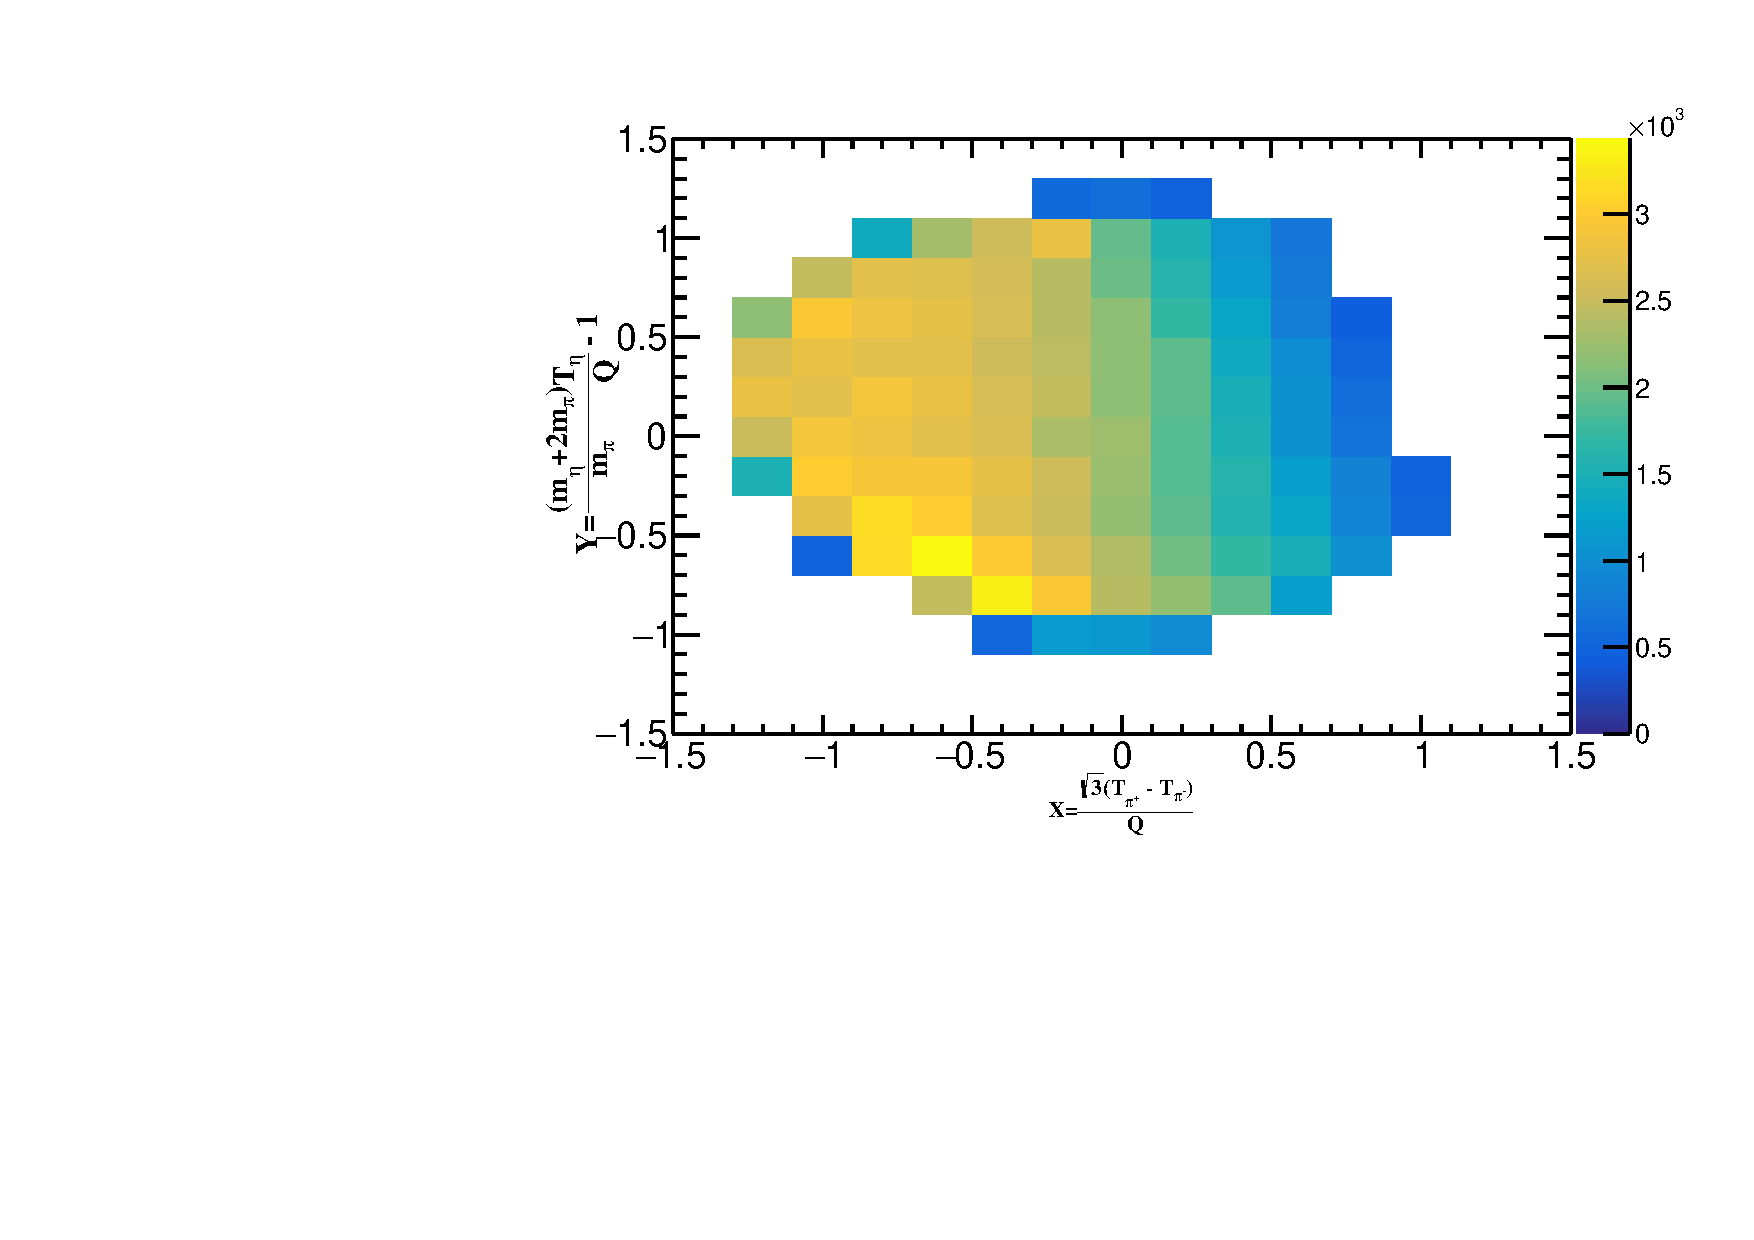
\includegraphics[width=10cm,height=6cm]{After_BS.pdf}}
\caption{Dalitz plot after background subtraction.}
\label{Af_DP}
\end{figure}

\begin{figure}
\centering
\begin{subfigure}{.5\textwidth}
  \centering
  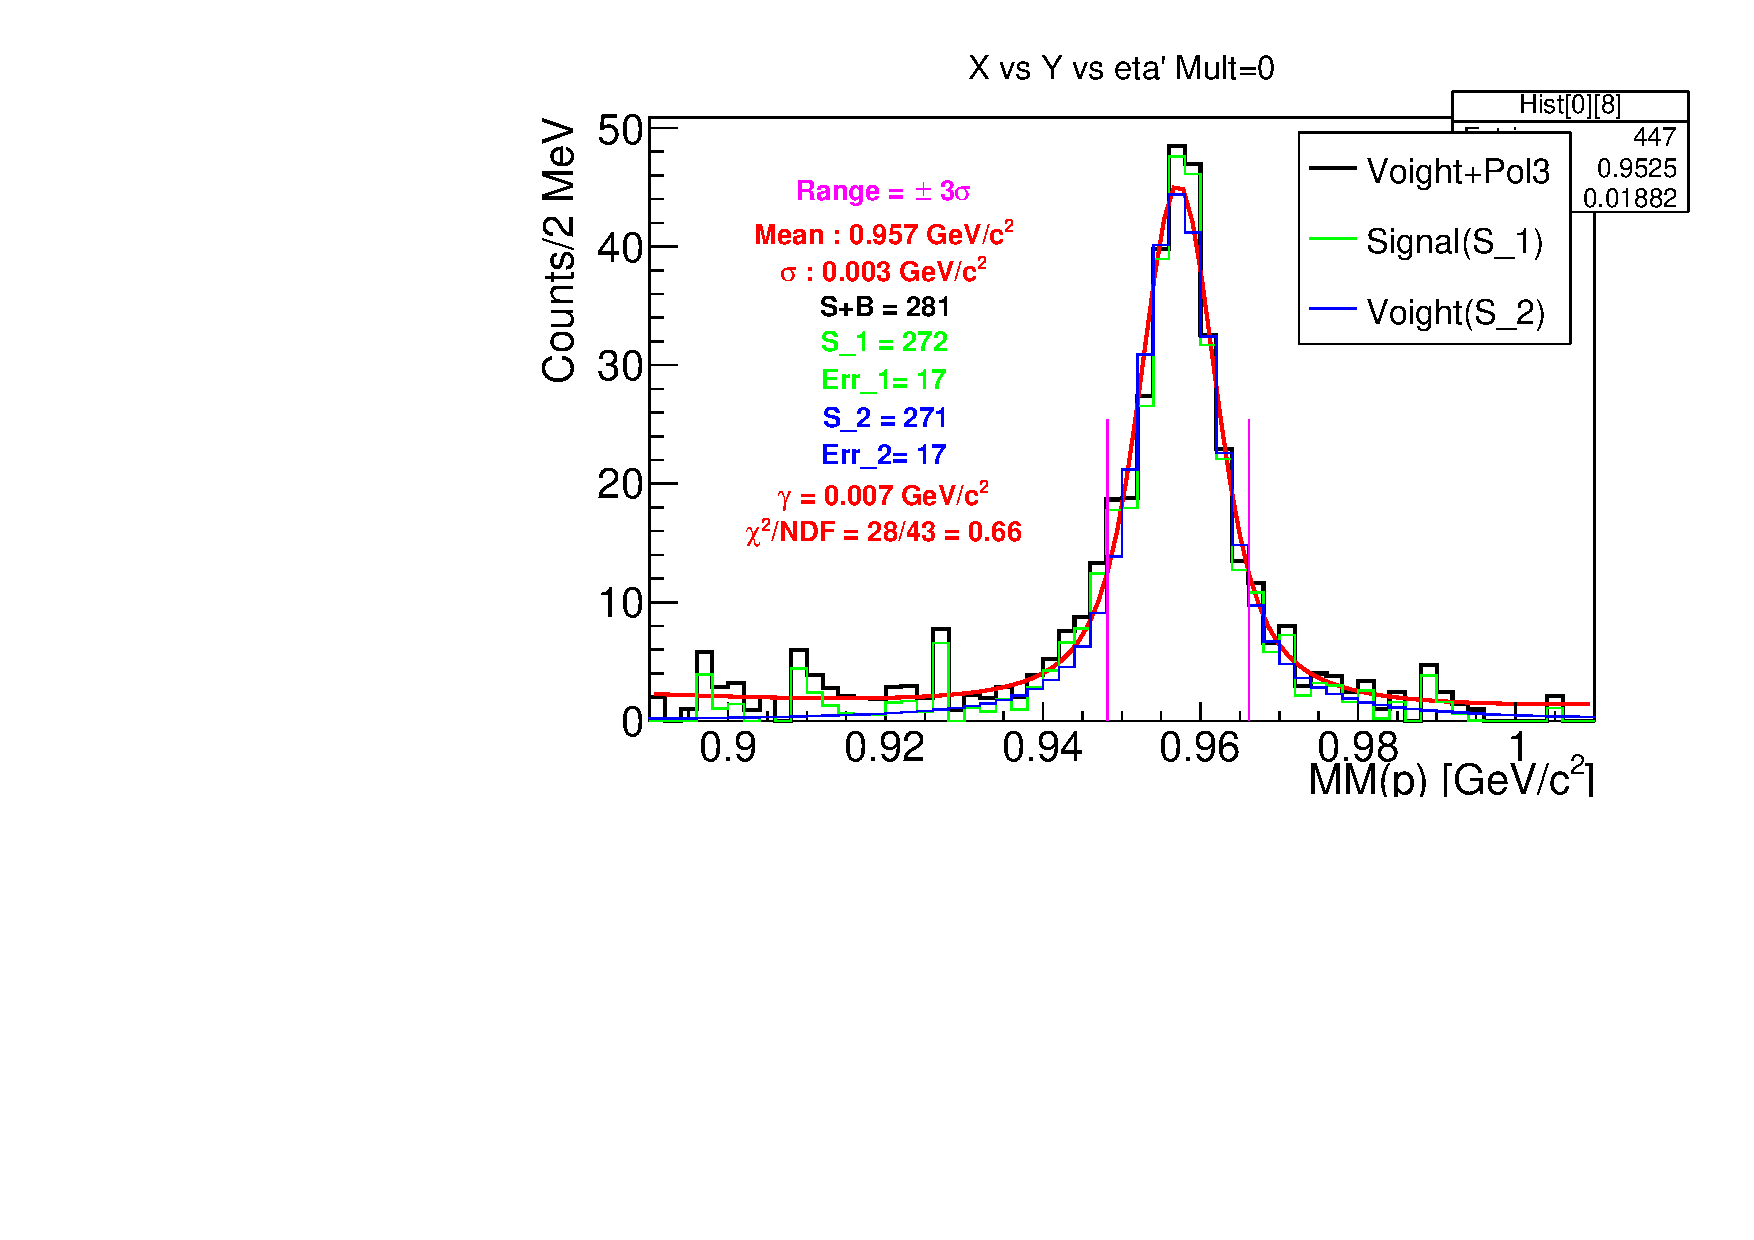
\includegraphics[width=.7\linewidth]{Hist[0][8].pdf}
  \caption{Fit to the $M_{x}$(p) distribution to a low statistics bin of Dalitz plot.}
  \label{fig:sub1}
\end{subfigure}%
\begin{subfigure}{.5\textwidth}
  \centering
  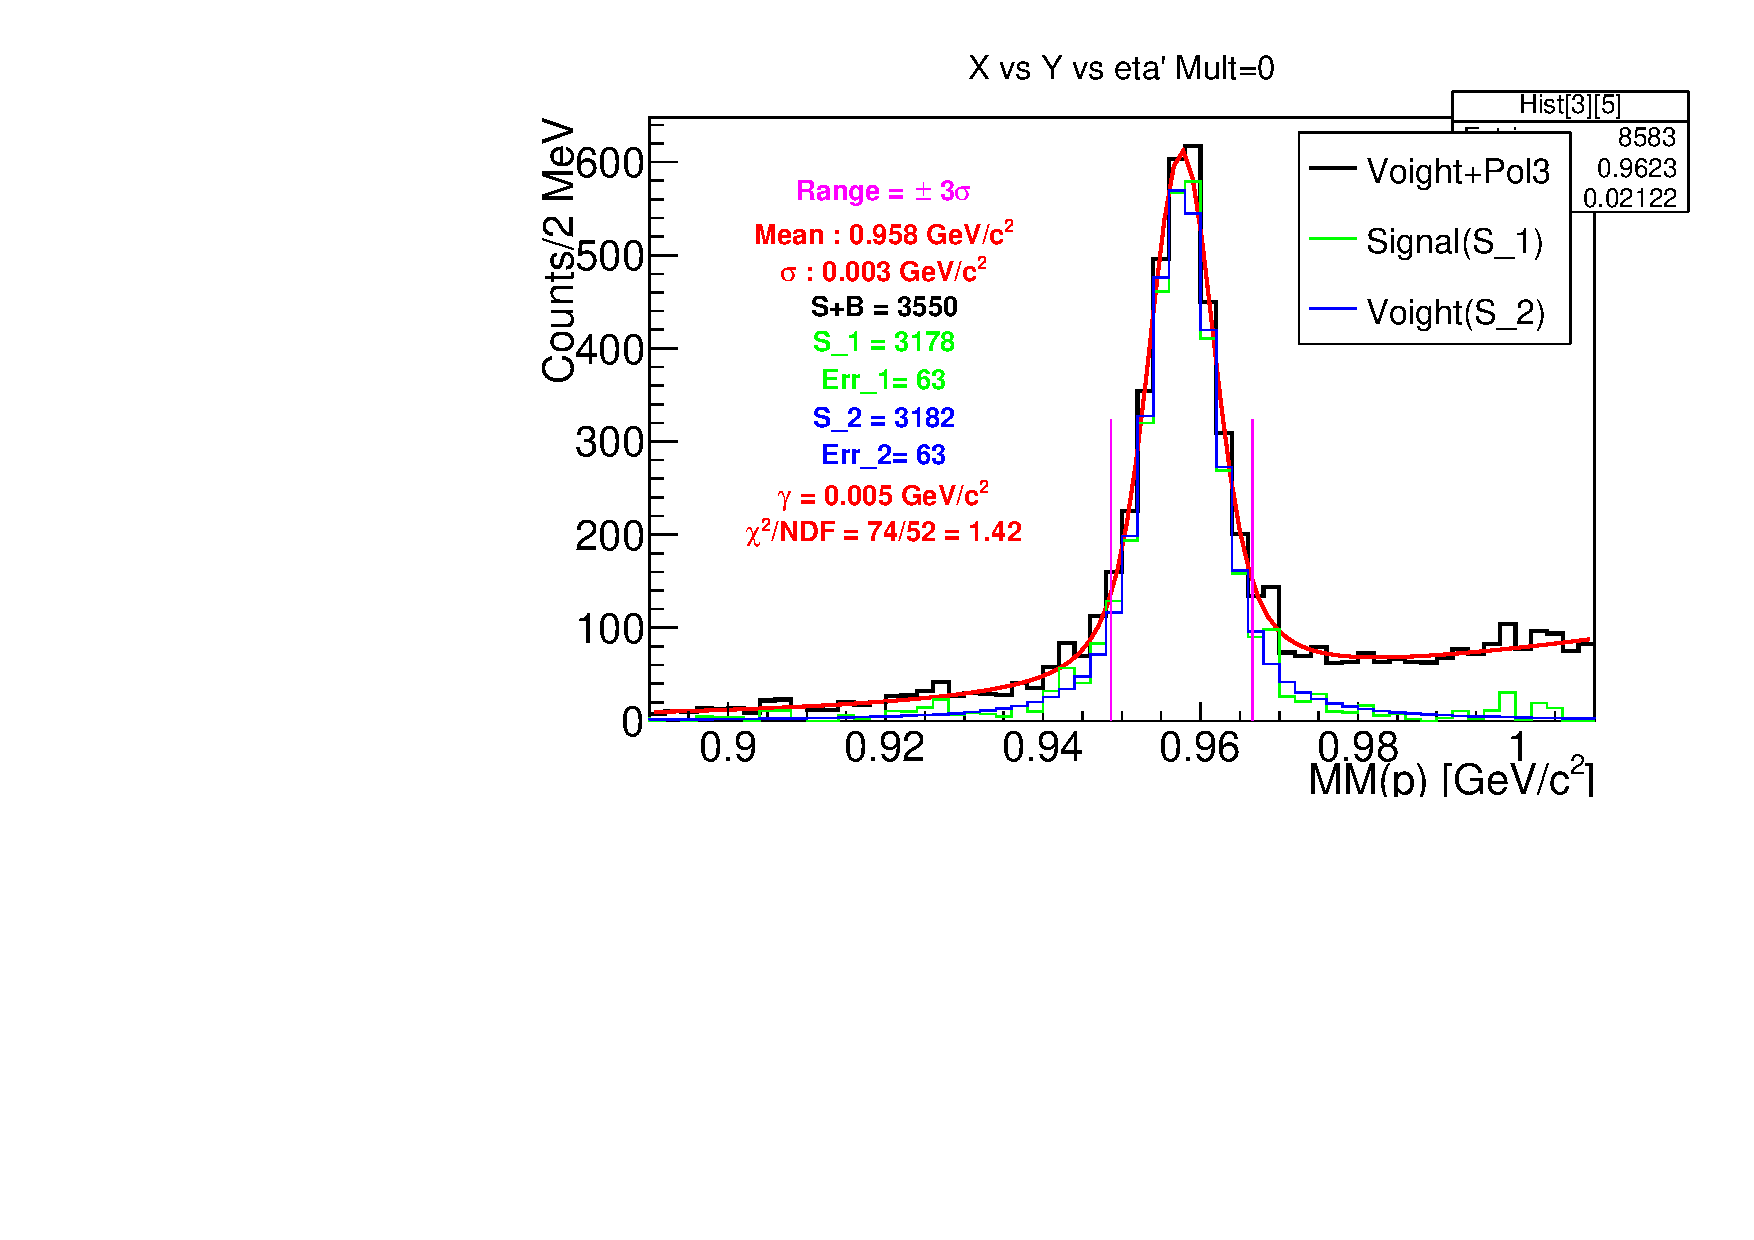
\includegraphics[width=.7\linewidth]{Hist[3][5].pdf}
  \caption{Fit to the $M_{x}$(p) distribution to a higher statistics bin of Dalitz plot.}
  \label{fig:sub2}
\end{subfigure}
\caption{A figure with two subfigures}
\label{DP_fit}
\end{figure}




One can also define the boundary of the $\eta^{\prime}$ $\rightarrow$ $\eta$ $\pi^{+}$ $\pi^{-}$ decay from the fact that the addition three momenta of particles $\vec{P}_{\eta}$, $\vec{P}_{\pi+}$ and $\vec{P}_{\pi-}$ for $\eta$, $\pi^{+}$ and $\pi^{-}$ respectively is 0 in the rest frame of $\eta^{\prime}$.
\begin{eqnarray*}
\vec{P}_{\eta} + \vec{P}_{\pi+} + \vec{P}_{\pi-} = 0.
\end{eqnarray*}
Squaring and equating the side gives us the boundary Equation.~\ref{bd} of the $\eta^{\prime}$ $\rightarrow$ $\eta$ $\pi^{+}$ $\pi^{-}$ decay.
\begin{eqnarray}
|{{P}_{\eta}}^2 - {{P}_{\pi+}}^2 - {{P}_{\pi-}}^2| \leq 2\vec{P}_{\pi+} . \vec{P}_{\pi-}
\label{bd}
\end{eqnarray}

One can also translate the 2D Dalitz plot bins of X and Y with a global bin number given by:
\begin{eqnarray*}
Globalbin(X,Y) = 
Floor \big[ \frac{X + X_{max}}{\delta} \big] + N_{bins} . Floor \big[ \frac{Y + Y_{max}}{\delta} \big] + 1
\label{gb}
\end{eqnarray*}
where X and Y are the central values of the current bin, $X_{max}$ and $Y_{max}$ are the maximum values the axis X and Y respectively, which is chosen to be 1.5. The $N_{bins}$ are the number of bins chosen along X and Y axis and it is 15 here. A translation of the Dalitz plot to its Global bin number along with the boundary of the decay from Equation.~\ref{bd} is shown in Figure.~\ref{fig10}. A global bin translation of the background subtracted Dalitz plot is shown in Figure.~\ref{DP_gl}.

\begin{figure}[ht!]
\centerline{
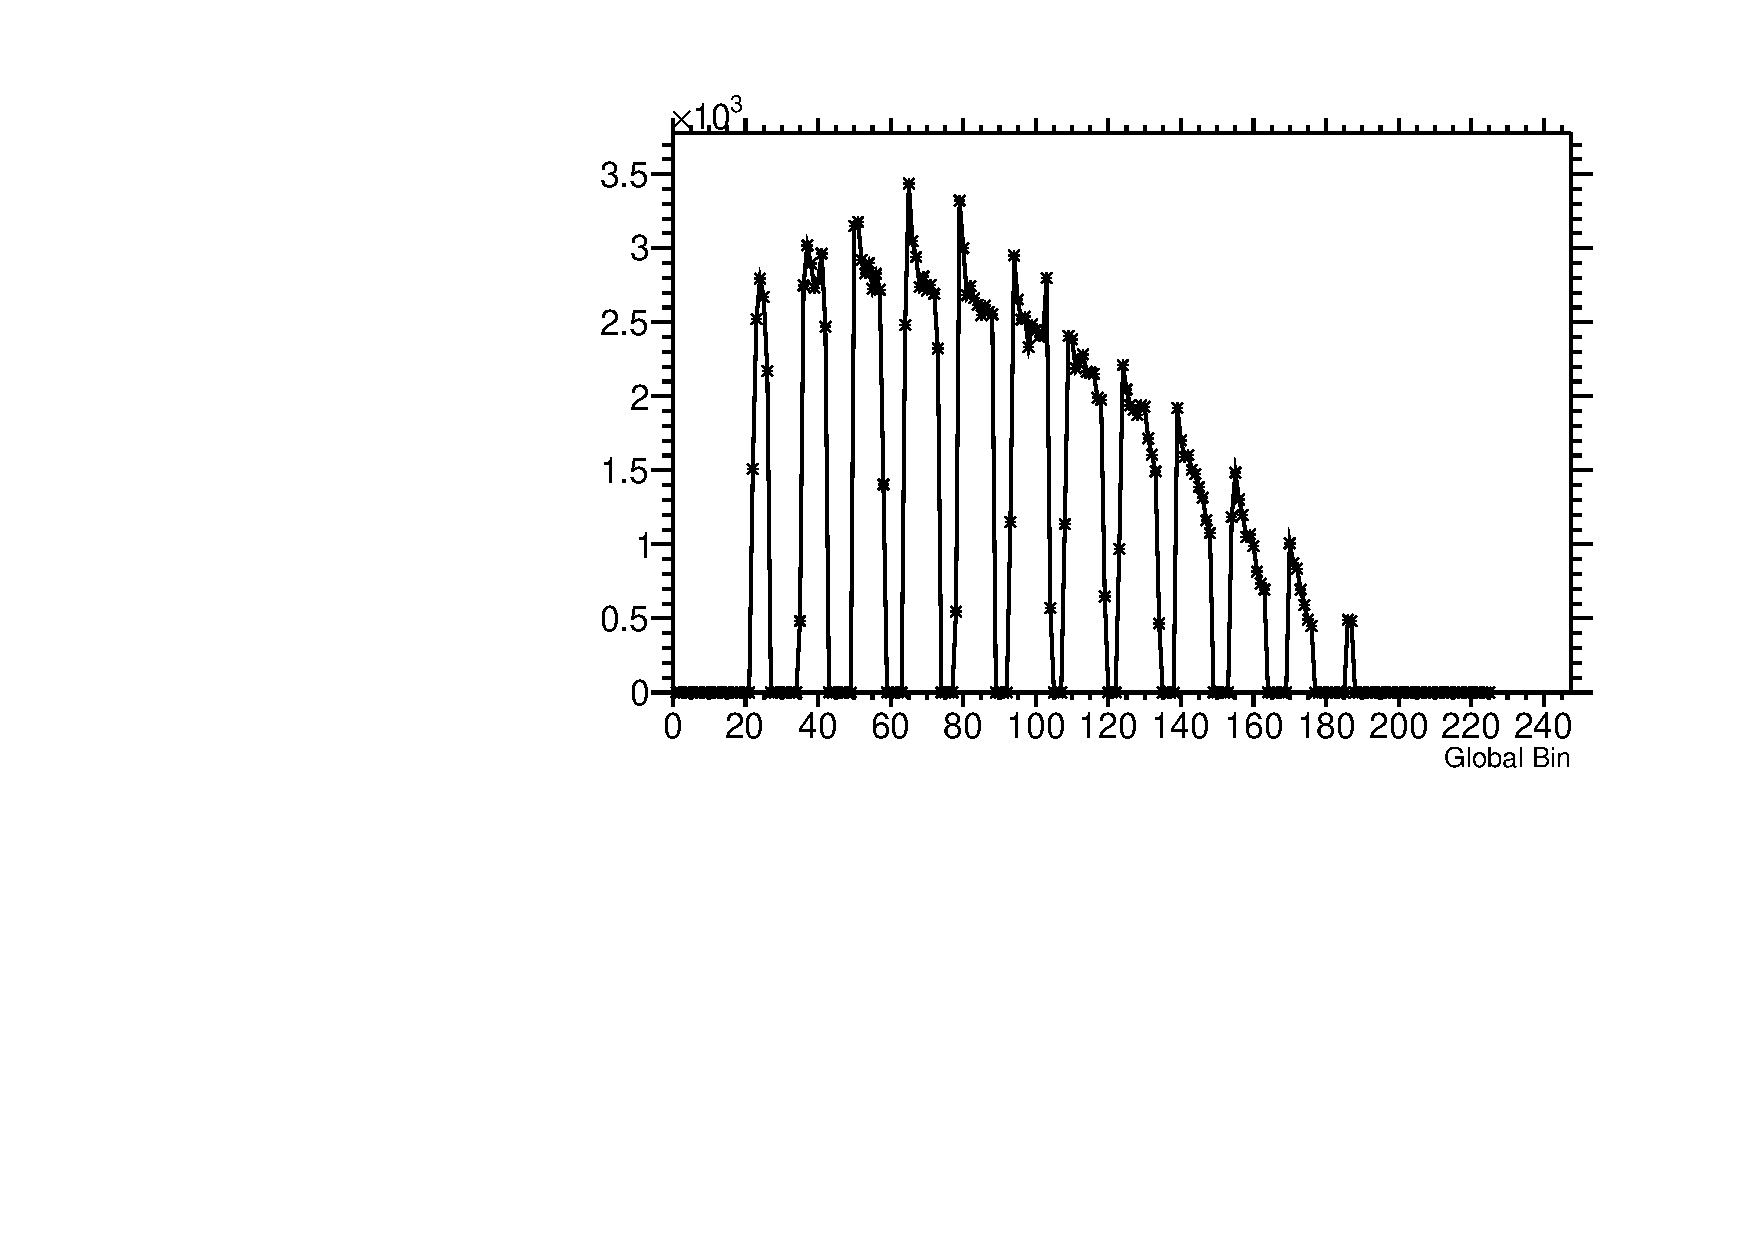
\includegraphics[width=10cm,height=6cm]{DP_Global.pdf}}
\caption{The background subtracted Dalitz plot in global bins.}
\label{DP_gl}
\end{figure}
 

%FIGURE OF DP WITH GLOBAL BIN
%FIGURE OF DATA DP WITH GLOBAL BIN
 
\begin{figure}[ht!]
\centerline{
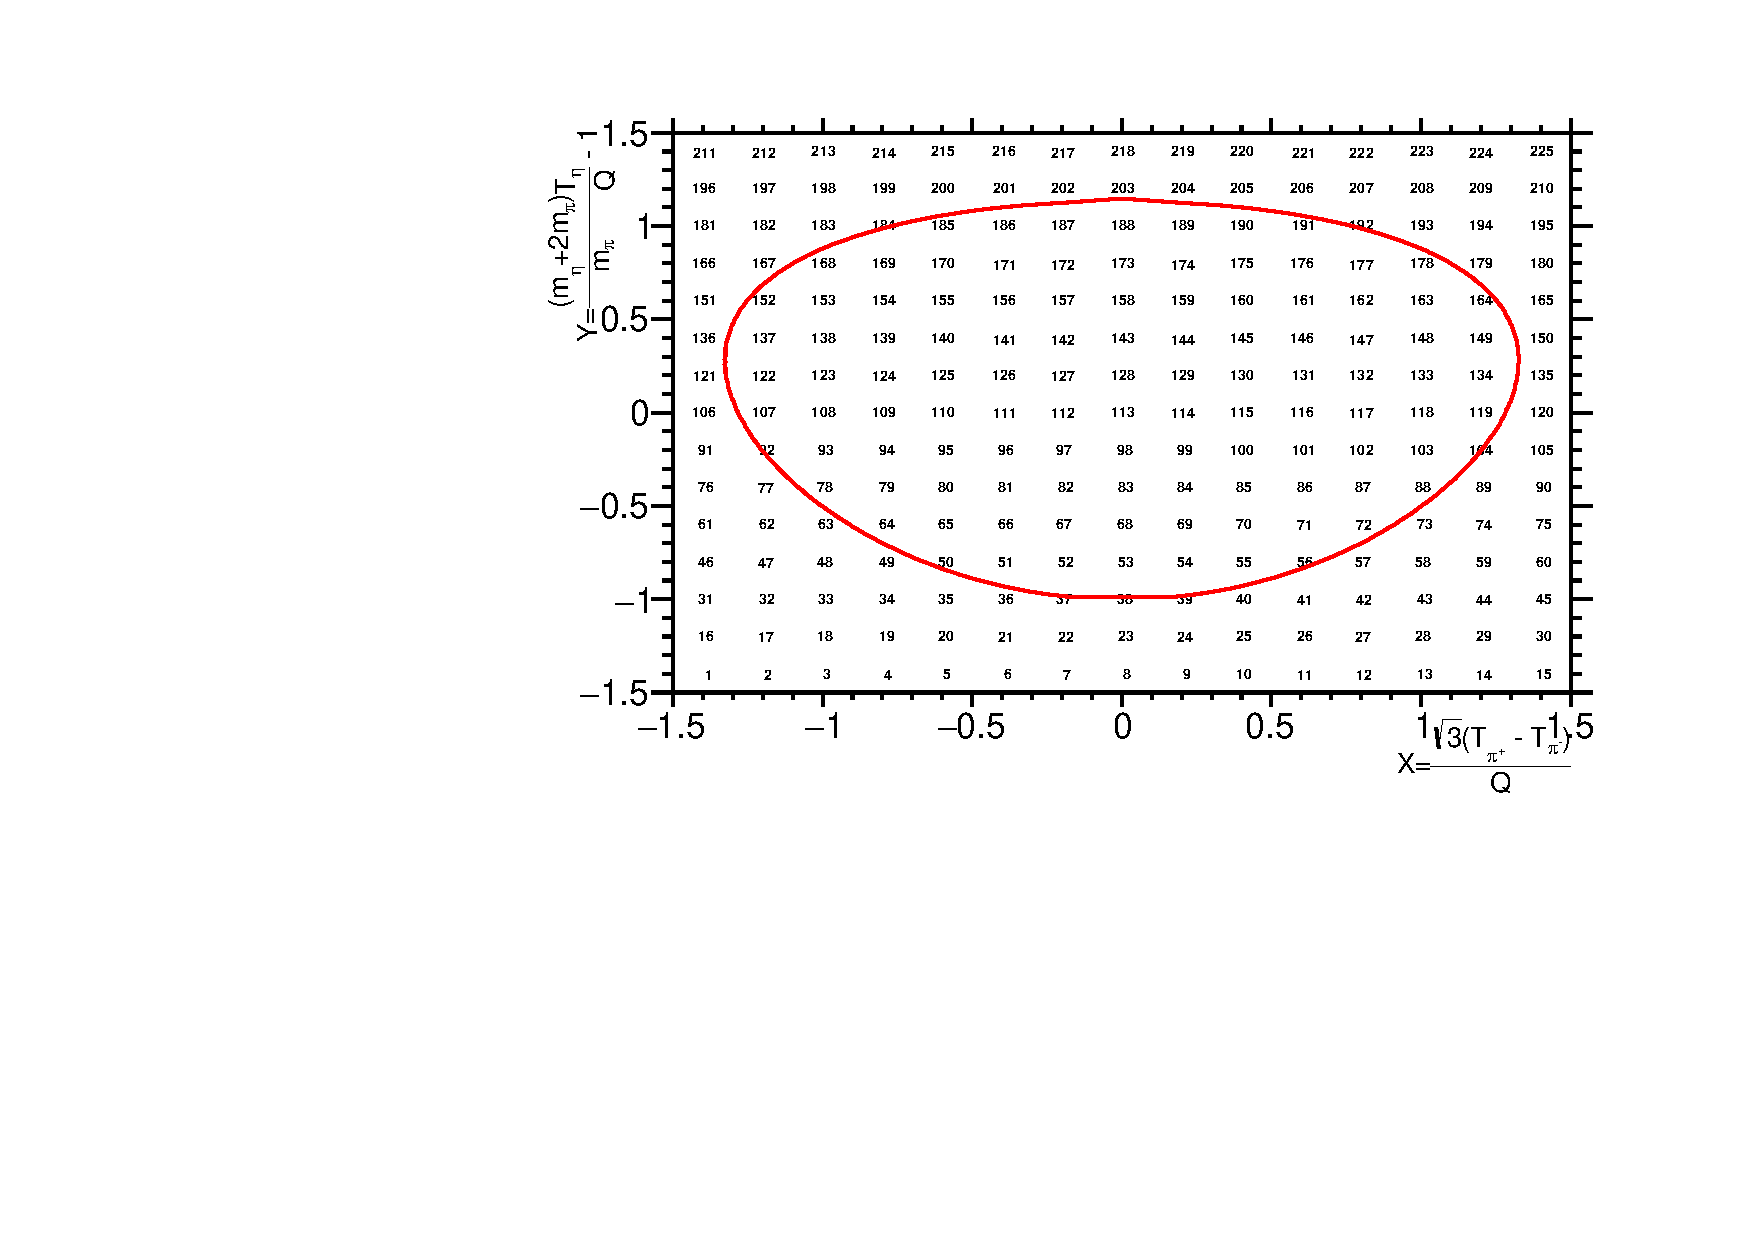
\includegraphics[width=14cm,height=8cm]{gb.pdf}}
\caption{The 15 x 15 Dalitz plot shows the translation X and Y Dalitz plot bins in global binning and the red curve shows the phase space boundary of the decay. }
\label{fig10}
\end{figure} 

 %FIGURE WITH 1D DP

\subsection{Calculation of acceptance with smearing matrix}

The CLAS detector has a different acceptance of proton, $\pi^{+}$ and $\pi^{-}$ and the acceptance varies within the phasespace of the  $\eta^{\prime}$ $\rightarrow$ $\eta$ $\pi^{+}$ $\pi^{-}$ decay. Hence the migration of events in different bins within the phasespace is also non-uniform, so one must take special care of migration of events from one bin to the other. To take care of the migration of the events,  an acceptance with smearing matrix ($\epsilon_{n,m}$) is presented here. The events are generated in each bin of the Dalitz plot and the acceptance for all the bins including the migrated bins are calculated. For events generated in the $j^{th}$ bin, the acceptance is calculated for all $i^{th}$ Dalitz plot bins as shown below :
\begin{eqnarray}
\epsilon_{i,j} = \frac{N_{rec,gen}(i,j)}{N_{gen}(j)}
\end{eqnarray}
Where $N_{rec,gen}$(i,j) denotes the number of events reconstructed in $i^{th}$ bin when generated events in the $j^{th}$ bin only.


\subsection{Fitting Procedure to the Dalitz Plot }

Once the $\eta^{\prime}$ $\rightarrow$ $\eta$ $\pi^{+}$ $\pi^{-}$ events from data is filled in each bin of Dalitz plot. We fit the Dalitz plot with the general parametization function in Equation.~\ref{par}. The square of the decay amplitude,
 \begin{equation}
M^{2}=A(1+aY+bY^{2}+cX+dX^{2}).
\label{par}
\end{equation}
Where a, b, c, and d are the Dalitz plot parameters of the decay and A is the normalization constant.

The fitting is performed with least square fitting procedure using MINUIT available in ROOT, which minimises the $\chi^{2}$ using Equation.~\ref{chi} in each bin of the Dalitz plot ~\cite{Caldeira}.
\begin{eqnarray}
\chi^{2} = \sum_{i=1}^{Nbins} \Bigg( \frac{N_{i} - \sum_{j=1}^{Nbins} \epsilon_{i,j} N_{theory,j}} {\sigma_{i}}   \Bigg)^{2}
\label{chi}
\end{eqnarray}
Where,
\begin {itemize}
\item The $N_{i}$ is number of $\eta^{\prime}$ $\rightarrow$ $\eta$ $\pi^{+}$ $\pi^{-}$ events in the $i^{th}$ Dalitz plot bin.
\item $\epsilon_{i,j}$ is acceptance with smearing matrix, ie.  it gives acceptance of $j^{th}$ bin when events are generated in the i$^{th}$ bin only.
\item $N_{theory,j}$ = $\int_{Boundary}$ A(1 + aY + b$Y^{2}$ + cX + d $X^{2}$) dX dY. 
\item $\sigma_{i}$ is the error associated with $i^{th}$ DP bin.
\end {itemize}

\subsubsection{Phase Space Integrals}

To calculate the integral in Equation.~\ref{Pi}, the Monte Carlo integration used within the boundary of the Dalitz plot. 
\begin{eqnarray}
N_{theory,j} = \int_{Boundary} A(1 + aY + b Y^{2} + cX + d X^{2}) dX dY
\label{Pi}
\end{eqnarray}
\begin{eqnarray*}
\begin{split}
\indent
N_{theory,j} = A \int_{Boundary} dX dY + A a \int_{Boundary} Y dX dY 
+ A b \int_{Boundary} Y^{2} dX dY \\ + A c \int_{Boundary} X dX dY 
+ A d \int_{Boundary} X^{2} dX dY 
\end{split}
\end{eqnarray*}
\begin{eqnarray*}
N_{theory,j} = A ( \alpha_{1} + a \alpha_{2} + b \alpha_{3} + c \alpha_{4} + d \alpha_{5})
\end{eqnarray*}
\noindent
Where,  
\indent
\\ $\alpha_{1}$ = $\int_{Boundary}$ dX dY
\indent
\\ $\alpha_{2}$ = $\int_{Boundary}$ Y dX dY
\indent
\\ $\alpha_{3}$ = $\int_{Boundary}$ $Y^{2}$ dX dY
\indent
\\ $\alpha_{4}$ = $\int_{Boundary}$ X dX dY
\indent
\\ $\alpha_{5}$ = $\int_{Boundary}$ $X^{2}$ dX dY

The aim here is to evaluate the integral $\alpha_{1}$, $\alpha_{2}$, $\alpha_{3}$, $\alpha_{4}$ and $\alpha_{5}$. The uniform random number pair, as Dalitz variable X and Y are generated within -1.5 to 1.5 for both using random number generator in ROOT and saved in a binned two dimensional histogram. If the generated pair lie inside the kinematic boundary of decay then the one binned two dimensional histogram for each integral is filled, where the integrand being the weight of the histogram.
For instance:  histogram for integral $\alpha_{1}$ is assigned a weight of 1, histogram for integral $\alpha_{2}$ is assigned a weight of Y, integral $\alpha_{3}$ is assigned a weight of $Y^{2}$ so on and so forth. These histograms for each integral is then divided by the generated histogram and multiplied by the bin size to give the value of integration inside the Dalitz plot for each bin. It can be later translated into the global binning and used directly in the Equation.~\ref{chi}.





\subsection{Results from the fit}
The fit results to general parametrisation to fit is shown below

 
\begin{center}
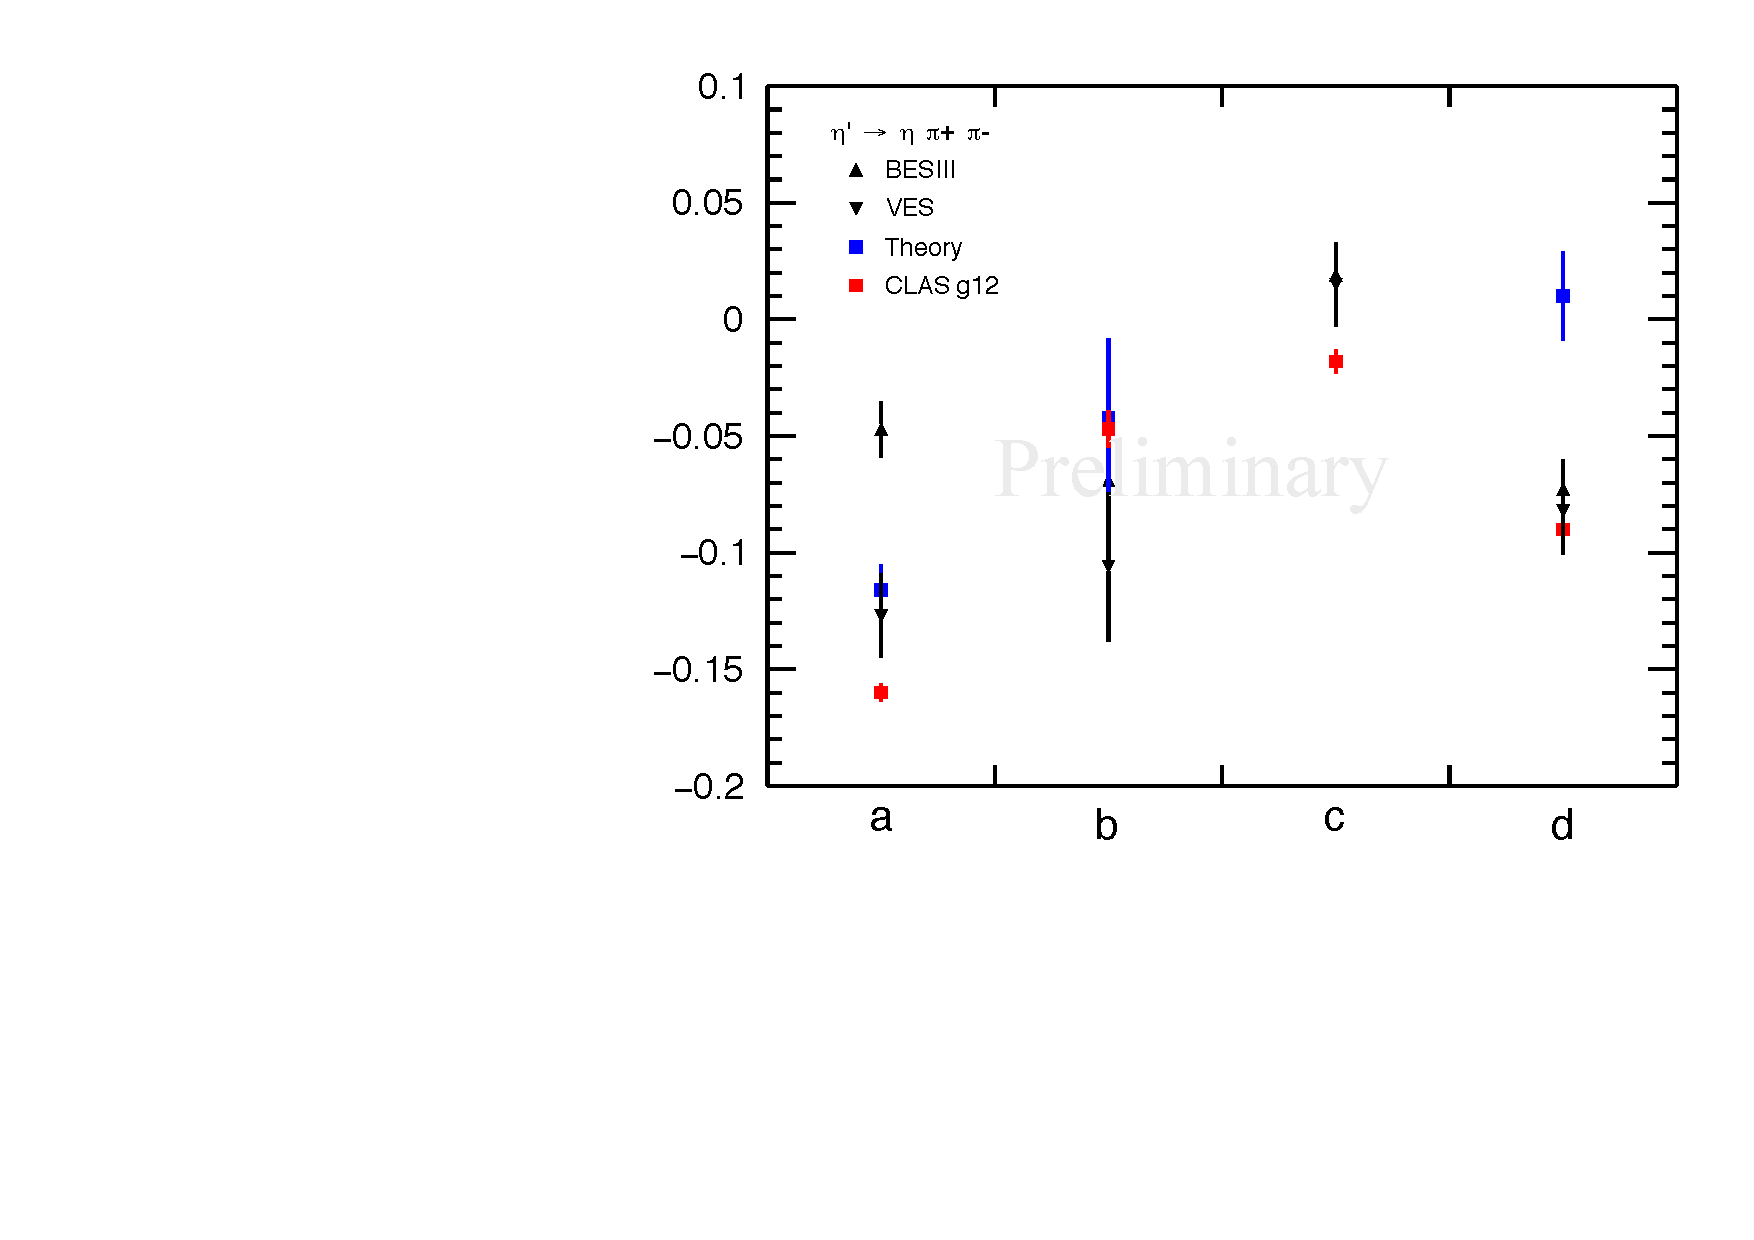
\includegraphics[width=10cm,height=5cm]{fit.pdf}
\end{center}

\begin{table}[!htb]
\centering
\begin{tabular}{|c|c|c|c|c|}
\hline
Parameter & {Theory [1]}           & VES [2]              & BESIII [3]          & { \textbf{Present Work}}   \\
\hline
a         & {-0.116 $\pm$ 0.011} & -0.127 $\pm$ 0.018 & -0.047 $\pm$ 0.012 & { \textbf{-0.160 $\pm$ 0.004}} \\
b         & {-0.042 $\pm$ 0.034} & -0.106 $\pm$ 0.032 & -0.069 $\pm$ 0.021 & { \textbf{-0.047 $\pm$ 0.008}} \\
c         & {...}              &{ 0.015 $\pm$ 0.018}  &{ 0.019 $\pm$ 0.012} & { \textbf{ -0.018 $\pm$ 0.005}} \\
d         & {+0.010 $\pm$ 0.019} & -0.082 $\pm$ 0.019 & -0.073 $\pm$ 0.013 & { \textbf{-0.090 $\pm$ 0.007}}  \\
\hline
$\frac{\chi^{2}}{NDF}$      &                                         & $\frac{129.3}{114}$ = 1.13                 & $\frac{504}{476}$ = 1.05                 & {$\frac{291}{97}$ = 3} \\
\hline
\end{tabular}
\end{table} 

%\begin {itemize}
%item I am sudeep
%\item N_{n} is no. of $\eta^{\prime}$ $\rightarrow$ $\eta$ $\pi^{+}$ $\pi^{-}$ events in the $n^{th}$ DP bin.
%\item $\epsilon_{n,m}$ is acceptance with smearing matrix, ie.  it gives acceptance of $m^{th}$ bin when events are generated in n$^{th}$ bin.
%\item $N_{theory,m}$ = $\int_{Boundary}$ A(1 + aY + bY^2 + cX + d X^2) dX dY
%\item $\sigma_{n}$ is the error associated with $n^{th}$ DP bin.
%\end{itemize}

\begin{thebibliography}{1}

%\cite{Dorofeev:2006fb}
\bibitem{Dorofeev:2006fb} 
  V.~Dorofeev {\it et al.},
   Phys.\ Lett.\ B {\bf 651}, 22 (2007)
   
\bibitem{Ablikim:2010kp} 
M.~Ablikim {\it et al.} [BESIII Collaboration],
Phys.\ Rev.\ D {\bf 83}, 012003 (2011)
   
%\cite{Borasoy:2005du}
\bibitem{Borasoy:2005du} 
  B.~Borasoy and R.~Nissler,
  %``Hadronic eta and eta-prime decays,''
  Eur.\ Phys.\ J.\ A {\bf 26}, 383 (2005)
     
\bibitem{G12_AN} 
 Z. Akbar et al. g12 Analysis Procedures, Statistics and Systematics. Technical report, CLAS Technical Note, 2016.

\bibitem{Williams:2009yj} 
  M.~Williams {\it et al.} [CLAS Collaboration],
  %``Differential cross s ections for the reactions gamma p ---> p eta and gamma p ---> p eta-prime,''
  Phys.\ Rev.\ C {\bf 80}, 045213 (2009)

\bibitem{Caldeira} 
Li Caldeira Balkeståhl, Measurement of the Dalitz Plot Distribution for $\eta$ $\rightarrow$ $\pi^{+}$ $\pi^{-}$ $\pi^{0}$ with KLOE, PhD thesis Uppsala University 2016. 

\end{thebibliography}
\end{document}
